\documentclass[12pt,number,sort&compress,preprint]{elsarticle}

%======================================================================

\usepackage{graphicx}
\usepackage{booktabs,multicol} %better tables
\usepackage{subcaption} %subfigs
\usepackage{lmodern}
\usepackage[T1]{fontenc}
\usepackage{textcomp}
\usepackage{gensymb}
\usepackage{ulem}

\usepackage{algorithm}
\usepackage[noend]{algpseudocode}

\usepackage[usenames,dvipsnames]{xcolor}

\usepackage[xcolor]{changebar}
\newcommand{\add}[1]{{\sloppy\cbcolor{teal}\textcolor{teal}{\cbstart {#1}\cbend}}}  % add
\newcommand{\delete}[1]{\sloppy\cbcolor{red}\textcolor{red}{\cbdelete\sout{#1}}}
\newcommand{\revise}[1]{{\sloppy\textcolor{Fuchsia}{#1}}}  % add

\newcommand{\addnl}[1]{{\sloppy\textcolor{teal}{#1}}}  % add
\newcommand{\deletenl}[1]{\sloppy\textcolor{red}{\sout{#1}}} %delete with no strikeout

% shared equations in separate file
% https://yatb.giacomodrago.com/en/post/3/latex-loading-equations-from-an-external-file.html
\usepackage{catchfilebetweentags}

% external references https://tex.stackexchange.com/a/14365/56227
\usepackage{xr-hyper}

\usepackage[version=4]{mhchem} % Formula subscripts using \ce{}, e.g., \ce{H2SO4}
\usepackage{amsmath,eqparbox,xparse,mathtools}
\usepackage[binary-units]{siunitx}

\usepackage{todonotes}

% load common macros / commands
\usepackage{macros}
% macro for small underscores for variable names in appendix
\usepackage{xspace}
\usepackage{relsize}
\newcommand{\smallunderscore}{\textscale{.5}{\textunderscore}\xspace}

\usepackage[breaklinks=true, linkcolor=blue, citecolor=blue, colorlinks=true]{hyperref}
% load after hyperref
\usepackage[english,capitalise]{cleveref}

% https://tex.stackexchange.com/a/146707/56227
\crefname{appendix}{}{}


%%%%%%%%%%%%%%%%%%%%%%%%%%%%
%      Custom Commands     %
%%%%%%%%%%%%%%%%%%%%%%%%%%%%


\sisetup{group-separator={,},
	detect-all,
	binary-units,
	list-units = single,
	range-units = single,
	range-phrase = --,
	per-mode = symbol-or-fraction,
	separate-uncertainty = true,
	multi-part-units = single,
	list-final-separator = {, and }
	%    scientific-notation = fixed
}

\DeclareSIUnit\doubles{doubles}

% load external document after hyperref https://tex.stackexchange.com/a/281417/56227
\externaldocument[deriv-]{derivations}

%======================================================================
% Add your bibliography file here, replace template.bib
\bibliographystyle{elsarticle-num}

% set figure path
\graphicspath{{./figures/}}


\title{Using SIMD and SIMT vectorization to evaluate sparse chemical kinetic Jacobian matrices and thermochemical source terms}

\author[1]{Nicholas Curtis\corref{corr}}
\author[2]{Kyle E.~Niemeyer}
\ead{nicholas.curtis@uconn.edu}
\author[1]{Chih-Jen Sung}

\address[1]{Department of Mechanical Engineering, University of Connecticut, Storrs, CT 06269, USA}
\cortext[corr]{Corresponding author}
\address[2]{School of Mechanical, Industrial, and Manufacturing Engineering, Oregon State University, Corvallis, OR 97331, USA}

\begin{document}

\begin{frontmatter}

%====================================================================
\begin{abstract} % not to exceed 200 words
A code generation platform, \texttt{pyJac}, for single-instruction, multiple-data (SIMD) and single-instruction, multiple thread (SIMT) vectorized \revise{constant-pressure\slash volume} thermochemical source-term and sparse\slash dense chemical kinetic Jacobian evaluation has been developed.% Can you introduce this a bit more? good to start with at least one sentence of introduction. also, this is passive and quite long\slash complex
Selected chemical kinetic models covering the range of sizes typically used in reactive-flow simulations were used for demonstration.
A new formulation of the chemical kinetic governing equations was derived and validated, \revise{resulting in} Jacobian sparsities of \SIrange{28.6}{92.0}{$\percent$} for the tested models.
Speedups of \SIrange{3.40}{4.08}{$\times$} were found for shallow-vectorized OpenCL source-rate evaluation \revise{compared with} a parallel OpenMP code on an \avx/ central processing unit (CPU), increasing to \SIrange{6.63}{9.44}{$\times$} and \SIrange{3.03}{4.23}{$\times$} for sparse and dense chemical kinetic Jacobian evaluation, respectively.
In addition, the performance of a Nvidia \gpunew/ graphics processing unit (GPU) was compared to a Nvidia \gpuold/ GPU finding speedups of \SIrange{1.40}{1.88}{$\times$}, \SIrange{1.10}{1.59}{$\times$}, and \SIrange{1.36}{3.0}{$\times$} for source-rate, sparse, and dense Jacobian evaluation, respectively. %is this sentence necessary in the abstract?
Furthermore, the effect of data-ordering was investigated and \revise{a} storage pattern specifically formulated for vectorized evaluation was proposed; as well, the effect of the \revise{constant pressure\slash volume} assumptions and varying vector widths were studied on source-term evaluation performance.
Speedups over a first-order finite-difference approach reached \SIrange{17.60}{45.13}{$\times$} and \SIrange{55.11}{245.63}{$\times$} for sparse\slash dense evaluation on the CPU \slash GPU respectively,%not sure what numbers refer to- sparse, dense, CPU, GPU?
while dense Jacobian evaluation was up to \SI{19.56}{$\times$} and \SI{2.84}{$\times$} times faster than a previous version of \texttt{pyJac} on a CPU and GPU, respectively.
Finally, future directions for vectorized chemical kinetic evaluation and sparse linear-algebra techniques were discussed.
\end{abstract}

% (Provide 2-4 keywords describing your research. Only abbreviations firmly
% established in the field may be used. These keywords will be used for
% sessioning/indexing purposes.)
\begin{keyword}
    Chemical Kinetics\sep SIMD\sep SIMT\sep Sparse\sep Jacobian
\end{keyword}

\end{frontmatter}
\todo[inline]{abstract comments in source}

%====================================================================
\section{Introduction}
%

\revise{As the combustion and reacting-flows community has recognized the
importance of detailed chemical kinetics for predictive reactive-flow simulations~\cite{LU2009192},
chemical kinetic models have grown in size and complexity to describe current and next-generation fuels relevant to transportation and power generation.
For example,} a recent biodiesel model~\cite{WESTBROOK2011742} consists of \textasciitilde\num{3500} chemical species and over \num{17000} reactions.
Moreover, the cost of evaluating the chemical source-terms scales linearly with the size of the model, while evaluating and factorizing the chemical kinetic Jacobian respectively scale quadratically and cubically with the number of species in the model, \revise{if naively implemented via a finite-difference method~\cite{LU2009192}}.
These factors often \revise{prohibit using} detailed chemical kinetics in practice; e.g., in a direct numerical simulation \revise{using} a 22-species model, \revise{evaluating} reaction rates consumed around half of the total run time~\cite{Spafford:2010aa}.
\revise{In addition, most common implicit integration techniques need to evaluate and factorize the Jacobian matrix to deal with stiffness.
As a result, these operations are bottlenecks when using even moderately sized chemical models in realistic reactive-flow simulations, necessitating other cost-reduction strategies~\cite{LU2009192}.}

A host of techniques have been developed to lessen the computational demand of chemical kinetic calculations while maintaining fidelity, \revise{falling} broadly into \revise{three} categories: removal of unimportant species and reactions~\cite{Lu:2006bb,Pepiot-Desjardins:2008,Hiremath:2010jw,Niemeyer:2010bt,Curtis:2015},
lumping of species with similar thermochemical properties~\cite{Lu:2007,Ahmed:2007fa,Pepiot:2008kq},
and time-scale methods that reduce numerical stiffness~\cite{Maas:1992ws,Lam:1994ws,Lu:2001ve,Gou:2010}.
\revise{We refer interested readers} to the recent review by Tur\'anyi and Tomlin~\cite{turanyi2016analysis} for a comprehensive overview.

In addition to the previously mentioned cost reduction methods, effort has gone into improving the integration algorithms and codes that evaluate the chemical kinetics~\cite{Gou:2010,SCHWER2002270,Niemeyer:2016aa,GAO2015287}.
In particular, a carefully derived analytical formulation of the Jacobian \revise{matrix can greatly increase sparsity}~\cite{SCHWER2002270} and drop the cost of Jacobian evaluation to \revise{linearly depend} on the number of species in the model~\cite{LU2009192}; \revise{sparse-matrix techniques can then reduce the cost of Jacobian factorization}~\cite{superlu99}.
\revise{In addition, studies have shown that} Single-Instruction, Multiple-Data (SIMD) and the related Single-Instruction, Multiple-Thread (SIMT) processors can accelerate chemical kinetic simulations~\cite{Shi:2012aa,Niemeyer:2014aa,Sewerin20151375,Niemeyer:2016aa,CurtisGPU:2017,stone2018}.

SIMD and SIMT programming are two important vector-processing paradigms used increasingly in scientific computing.
Traditional multi-core parallelism is often used to increase central processing unit (CPU) performance; however, as exponential growth in processing power---colloquially known as Moore's law---has slowed~\cite{khan2018science}, SIMD processors as well as SIMT processors, e.g., in the form of graphics processing units (GPUs), have gained recognition due to their increased floating operation throughput.\todo{this isn't quite right; multicore parallelism is how CPUs have bypassed Moore's}{}
The parallel programming standard OpenCL~\cite{stone2010opencl} has further enabled adoption of vector processing in scientific computing by providing a common application program interface (API) for execution on heterogeneous systems, e.g., CPU, GPU, or Intel's Many Integrated Core (MIC) architecture.
\revise{Here we will} largely use OpenCL terminology to describe these processing paradigms, as it provides a convenient way to classify otherwise disparate processor types (e.g., CPUs and GPUs).
However, the concepts discussed herein \revise{broadly apply} to SIMD\slash SIMT processing.

\begin{figure}[htb]
  \centering
  \begin{subfigure}[t]{0.45\linewidth}
      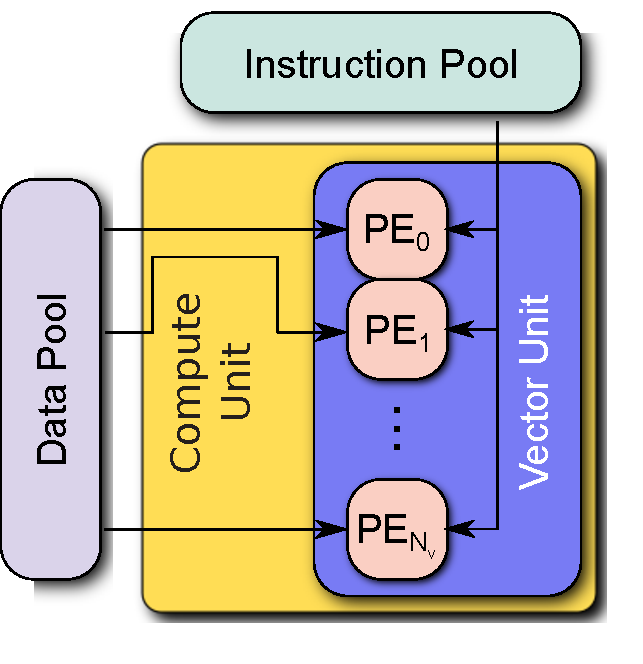
\includegraphics[width=\textwidth]{SIMD.pdf}
      \caption{Schematic of SIMD processing.  A single compute unit (e.g., a CPU core) contains a vector unit with $N_v$ processing elements (PEs), together called a vector-lane.  The vector unit executes a single instruction concurrently on multiple data.}
      \label{F:SIMD}
  \end{subfigure}
  \hfill
  \begin{subfigure}[t]{0.45\linewidth}
      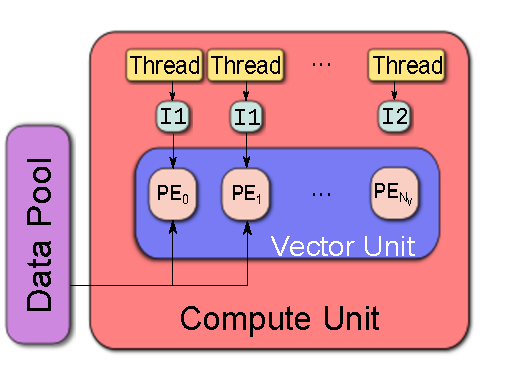
\includegraphics[width=\textwidth]{SIMT.pdf}
      \caption{Schematic of SIMT processing. A single compute unit (e.g., a GPU streaming multiprocessor) contains many processing elements (PEs) and hosts many threads, each with an instruction to execute (I1, I2).  Threads with the same instruction execute concurrently on multiple data while the others must wait (leading to thread divergence).}
      \label{F:SIMT}
  \end{subfigure}
  \caption{Simple diagrams explaining the fundamentals of the SIMD and SIMT vector-processing paradigms.}
\end{figure}

A typical modern CPU \revise{contains multiple} compute units (i.e., cores), each with specialized vector processing units capable of running SIMD instructions, \revise{as \cref{F:SIMD} depicts}.
A SIMD instruction uses the vector processor to execute the same floating-point operation (e.g., multiplication, division) \revise{on different data} concurrently.
\revise{The vector-width is the number of possible concurrent operations, typically around two to four in double precision.}\footnote{OpenCL allows for use of vector-widths different from the actual hardware vector-width via implicit conversion, and may provide some performance benefit as Sec.~\ref{S:results} \revise{discusses.}}
Specialized hardware accelerators \revise{have also been developed, like Intel's Xeon Phi co-processor (i.e., the MIC architecture)}, that have tens of cores with wide vector-widths (e.g., \numrange{4}{8} double-precision operations).
\revise{Cutting-edge and forthcoming Intel CPUs also include these wide vector-widths, like the Skylake Xeon and Cannon Lake architectures.}

\revise{Modern GPUs rely on the related computing paradigm of SIMT processing, where a single compute element hosts large
numbers of threads (a streaming multiprocessor in Nvidia terminology)~\cite{lindholm2008Nvidia}.}
\revise{\Cref{F:SIMT} depicts a SIMT compute unit, where a group of threads---typically \num{32}, known as a warp on Nvidia GPUs---execute the same SIMT instruction on multiple data concurrently}.
If some threads must execute a different instruction, they are forced to wait and execute later; \revise{this may occur due to if\slash then branching or predication.}
This phenomenon, known as thread-divergence, is a key consideration for SIMT processing and can cause serious performance degradation for complicated algorithms~\cite{CurtisGPU:2017}.

\subsection{Related work}
\label{S:related}


Recognizing the need to accelerate chemical-kinetic Jacobian evaluation and factorization, a number of recent works have been published on \revise{constructing analytical Jacobian matrices}; although as will be discussed at the end of this section, \revise{here we offer} several key improvements over past efforts.
\add{Schwer et al.~\cite{SCHWER2002270} were among the first to recognize the critical importance of a sparse analytical Jacobian to accelerate chemical kinetic simulations.}
\revise{Later, Safta et al.~\cite{Safta:2011vn} developed the \texttt{TChem} software package}, which was one of the first developed that provides analytical Jacobian evaluation. However, \texttt{TChem} has several limitations, including incompatibility with modern reaction types---i.e., pressure dependent Arrhenius (or P-Log) and Chebyshev reactions---and its lack of thread-safety to enable parallel execution~\cite{Curtis2017:tchem}.
Youssefi~\cite{Youssefi:2011tm} explored the importance of analytical Jacobian matrices for time-scale analysis techniques as well as their effect on computational efficiency in zero-dimensional homogeneous reactor simulations.
Bisetti~\cite{Bisetti:2012jw} developed an isothermal, isobaric analytical Jacobian code-generation utility;
\revise{this approach significantly increases Jacobian sparsity, although the chosen isothermal assumption is not typical in most combustion simulations.}
In the same work Bisetti \revise{also} provided a novel way to compute dense matrix-vector multiplications resulting from a change of system variables without \revise{storing} the full Jacobian.
Perini et al.~\cite{Perini:2012gy} developed an analytical Jacobian code for constant-volume combustion, with additional options to increase sparsity (at the expense of strict correctness) and \revise{tabulate} temperature-dependent properties; \revise{they reported} an \SI{80}{\percent} speedup over a finite-difference-based Jacobian when used in a multidimensional reactive-flow simulation.
Gao et al.~\cite{GAO2015287} derived a sparse analytical Jacobian, but did not validate it outside the context of use with an implicit-integration technique.
In addition, since the Jacobian was based on an over-constrained system~\cite{HANSEN2018257}, the effect on strict conservation of mass\slash energy was not studied.

\revise{Recently, some groups have developed frameworks for constructing analytical Jacobians for evaluation on modern SIMD or SIMT processors.}
Dijkmans et al.~\cite{Dijkmans:2014bb} developed a GPU-based analytical Jacobian code with optional tabulation of temperature-dependent properties, and \revise{showed} speedups up to \SI{120}{$\times$} for zero-dimensional chemical kinetic integration with large chemical models (\textasciitilde\num{3000} species).
\add{Bauer et al.~\cite{Bauer:2014} used warp-specialization to improve GPU-vectorization over a standard data-parallel vectorization approach; they achieved speedups of up to \SIrange{2.81}{3.75}{$\times$}, \SIrange{1.91}{2.58}{$\times$}, and \SIrange{1.4}{1.5}{$\times$} for evaluating viscosity, species diffusion, and chemical source terms, respectively}.
Niemeyer et al.~\cite{Niemeyer:2016aa} created and validated the open-source analytical chemical kinetic Jacobian code-generator, \texttt{pyJac}, which supports parallel execution on CPUs and SIMT execution on GPUs; \revise{\texttt{pyJac} enables} a speedup of \SIrange{3}{7.5}{$\times$} over a finite-difference Jacobian on the CPU.

\add{Relevant to all of the aforementioned efforts, Hansen and Sutherland~\cite{HANSEN2018257} explored the choice of thermochemical state vectors and the resulting effect on consistency and errors in conserved properties such as mass and energy.
They also characterized how the choice of state vector affects implicit\slash linearly implicit integration algorithms and chemical mode analysis techniques.
Overall they found that while many literature Jacobian formulations are not strictly correct or over-specified, such flaws negligibly affect Newton--Krylov methods---perhaps because the incorrect Jacobian reasonably approximates the true Jacobian.
On the other hand, linearly implicit algorithms like Rosenbrock methods and analysis techniques like chemical explosive mode analysis~\cite{lu_yoo_chen_law_2010} need accurate and correct Jacobians.
}

A number of recent works have investigated \revise{using} high-performance SIMT devices \revise{like GPUs} to accelerate reactive-flow and chemical kinetics simulations.
Spafford et al.~\cite{Spafford:2010aa} coupled GPU-based chemical source-term evaluation with an explicit direct numerical simulation code, achieving an order of magnitude speedup \delete{on a Tesla C1060} compared to a \add{CPU-based} serial implementation \delete{on a AMD-Opteron processor}.
Shi et al.~\cite{Shi:2011aa} combined GPU-based chemical kinetic source-term evaluation and Jacobian factorization with two implicit CPU solvers, achieving an order-of-magnitude speedup for homogeneous reactor simulations of large chemical models\delete{on a Tesla 2050 GPU} over a serial\delete{Intel i7 930} CPU implementation.
Niemeyer et al.~\cite{Niemeyer:2011aa} implemented an explicit solver for non-stiff chemistry on a Tesla C2075 GPU, achieving a speedup of nearly two orders of magnitude over a sequential \add{CPU} code\delete{on an Intel Xeon X5650 CPU}.
Shi et al.~\cite{Shi:2012aa} proposed a strategy for chemical-kinetic integration in three-dimensional reactive-flow simulations, where a traditional implicit integrator handled the stiffest computational cells on a CPU and a stabilized-explicit solver \delete{on a Tesla C2050 GPU} solved the less-stiff cells on a GPU; this hybrid solution technique \revise{performs} \SIrange{11}{46}{$\times$} faster than the implicit CPU solver alone for simulation of a premixed diesel engine.
Le et al.~\cite{Le2013596} found a \SIrange{30}{50}{$\times$} speedup for a GPU-based shock-capturing reactive-flow code\delete{ on a Tesla C2070} as compared with a sequential \add{CPU} version of the same\delete{on an Intel Xeon X5650 CPU}.
Stone and Davis~\cite{Stone:2013aa} investigated a GPU-based version of a common implicit integrator (VODE~\cite{Brown:1989vl}), finding an order-of-magnitude speedup over a serial CPU implementation.
Niemeyer and Sung~\cite{Niemeyer:2014aa} developed a GPU-based stabilized explicit integrator for use with moderately-stiff chemical kinetics, achieving an order of magnitude speedup\delete{on a Tesla C2075 GPU} over a multithreaded VODE solver on a six-core\delete{Intel X5650} CPU.
Sewerin and Rigopoulos~\cite{Sewerin20151375} studied a fifth-order implicit Runge--Kutta solver on both consumer-grade and high-end GPUs\slash CPUs; the high-end GPU solver was at best \SI{1.8}{$\times$} slower than the high-end CPU version running on \num{16} cores.
Yonkee and Sutherland~\cite{Yonkee2016} implemented GPU-accelerated evaluations of thermodynamic parameters, multicomponent transport properties, and species production rates for solving partial differential equations (PDEs) \delete{on an Intel Xeon E5-2680} \add{both the CPU} and \delete{a Tesla K20} GPU.
In evaluating the thermochemical properties, speedups between \SIrange{8}{13}{$\times$} were found (over a serial version of the same code) while running on 16 CPU cores, and \SIrange{20}{40}{$\times$} on the GPU; they showed speedups of \textasciitilde\SI{9}{$\times$} and \textasciitilde\SI{25}{$\times$} when simulating a partially premixed methanol flame PDE on 16 CPU cores and the GPU, respectively.\todo{revise this sentence, fairly awkward}{}
Curtis et al.~\cite{CurtisGPU:2017} implemented a fifth-order implicit Runge--Kutta method~\cite{wanner1991solving}, as well as two fourth-order exponential integration techniques~\cite{Hochbruck:1998,Hockbruck:2009} paired with an analytical Jacobian code~\cite{Niemeyer:2016aa} \delete{on a Tesla C2075} \add{on the GPU and CPU}.
The \add{GPU-based} implicit Runge--Kutta method performs equivalently to a standard implicit integrator~\cite{Hindmarsh:2005} running on \numrange{12}{38} \delete{Intel Xeon E5-4640 v2} CPU cores for two relatively small chemical models \delete{with an integration time step of $10^{-6}$ s}.

In contrast, SIMD-based chemical kinetics evaluation\slash integration have been studied far less.
Linford et al.~\cite{Linford:2011} implemented a three-stage, second-order Rosenbrock integrator for atmospheric chemical kinetics on the CPU, GPU, and cell broadband engine (CBE)---a specially designed vector processor---and found speedups regularly exceeding~\SI{25}{$\times$} over a serial CPU implementation.
Kroshko and Spiteri~\cite{kroshko2013efficient} implemented a SIMD-vectorized third-order stiff Rosenbrock integrator for atmospheric chemistry on the CBE and found a speedup of \SI{1.89}{$\times$} (a parallel scaling efficiency of \SI{94}{$\percent$}) over a serial version of the same code.
Stone et al.~\cite{stone2018} implemented a linearly-implicit fourth-order stiff Rosenbrock solver in the OpenCL for various platforms including CPUs, GPUs, and MICs.
They found that SIMD vectorization improves integrator performance over an OpenMP baseline vectorized by simple compiler hints (i.e., \texttt{\#pragmas}) by \SIrange{2.5}{2.8}{$\times$} on the CPU and \SIrange{4.7}{4.9}{$\times$} on the MIC, while the GPU performs only \SIrange{1.4}{1.6}{$\times$} faster than the OpenMP baseline due to thread divergence~\cite{stone2018}.


\subsection{Goals of this study}
\label{S:Goals}

This work builds upon our previous analytical chemical kinetic Jacobian code, \texttt{pyJac}~\cite{Niemeyer:2016aa}.
In this article we
\begin{itemize}
 \item Derive and validate a new Jacobian formulation for \texttt{pyJac} that greatly increases sparsity;
 \item Enable cross-platform SIMD\slash SIMT vectorization for CPUs, GPUs, and other accelerators;
 \item Investigate the performance for a wide range chemical kinetic models, specifically looking at speedups due to SIMD\slash SIMT-vectorization as well as relative to the previous version of \texttt{pyJac}; and finally
 \item Discuss future extensions to this work as well as several promising directions for SIMD\slash SIMT vectorization in reactive-flow simulations.
\end{itemize}
To our knowledge, this is the first \add{open-source, validated} effort that vectorizes the evaluation of chemical-kinetic source terms and Jacobian matrices for any chemical model on a wide selection of platforms.

\section{Methodology}
\subsection{Data ordering and vectorization patterns}
\label{S:data}

\begin{figure}[htb]
  \centering
  \begin{minipage}{0.45\linewidth}
    \begin{subfigure}[t]{\textwidth}
      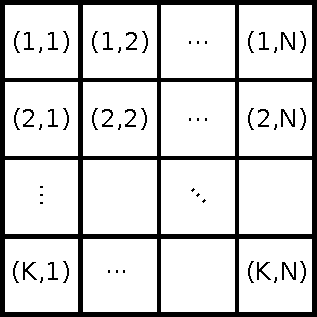
\includegraphics[width=\textwidth]{data_layouts.pdf}
      \caption{A simple 2-D data array with K rows and N columns.}
      \label{F:mem}
    \end{subfigure}
  \end{minipage}
  \hfil
  \begin{minipage}{0.45\linewidth}
    \begin{subfigure}[t]{\textwidth}
	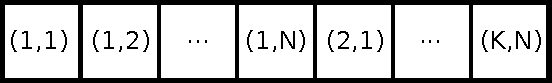
\includegraphics[width=\textwidth]{row_major.pdf}
	\caption{Row-major data ordering}
	\label{F:row_major}
    \end{subfigure}
    \\
    \\
    \\
    \\
    \begin{subfigure}[t]{\textwidth}
	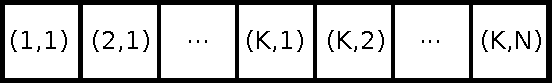
\includegraphics[width=\textwidth]{column_major.pdf}
	\caption{Column-major data ordering}
	\label{F:column_major}
    \end{subfigure}
  \end{minipage}
  \caption{\addnl{Simple data-layout patterns for 2-D arrays}}
\end{figure}

When storing arrays for a chemical kinetic model, the data-storage layout and vectorization patterns are critical to achieving high-performance code.
\Cref{F:mem} depicts an example data array with $K$ rows and $N$ columns \revise{where} index ($i$, $j$) \revise{corresponds} to the $i$th row and $j$th column.
For example, the concentration of species $j$ for the $i$th thermochemical state would be stored in $[C]_{i, j}$ with $1 \le i \le N_{\text{state}}$ (the number of thermochemical states considered for evaluation) and $1 \le j \le \ns/$ (the number of species in the model).
The stored concentrations would then have $K = N_{\text{state}}$ rows and $N = \ns/$ columns.

The ``C'' (C row-major) format stores the concentrations of all species for a single thermochemical condition $i$  sequentially in memory, i.e., with  $[C]_{1, 1}$ in index 1, $[C]_{1, 2}$ in index 2, and so on, as shown in \cref{F:row_major}.\todo{wouldn't these start at index 0?}{}
Conversely, in the ``F'' (Fortran column-major) format the concentrations of a single species $j$ over all thermochemical states lie adjacent in memory, corresponding to storing $[C]_{1, 1}$ in index 1, $[C]_{2, 1}$ in index 2, and so on, as shown in \cref{F:column_major}.
This ordering \revise{strongly affects} the performance of SIMD\slash SIMT-vectorized algorithms, \revise{as does the device (CPU, GPU, etc.\@) and vectorization pattern in question.}

In a \textit{shallow}-SIMD\slash SIMT vectorization (also referred to as ``per-thread'' in previous works using GPUs~\cite{Stone:2013aa}), each SIMD lane (or SIMT thread) in a compute unit evaluates the source terms or Jacobian for a different thermochemical state.
If the data is stored in ``F''-order, the SIMD-lanes\slash SIMT-thread accessing $[C]_{1, j}\ldots[C]_{N_v, j}$---the concentration of species $j$ for states $1, 2,\ldots N_v$, where $N_v$ is the SIMD vector-width or the number of threads in a SIMT warp---will load sequential locations in memory.
The first $(j+1)$th species concentration, $[C]_{1, j+1}$, will be $N_{\text{state}}$ memory locations away; this increases the likelihood of cache-misses on the CPU~\cite{gray2000rules}, but conversely is well suited to coalesced memory accesses on the GPU~\cite{Nvidia:2018}.

In a \textit{deep}-SIMD\slash SIMT vectorization (also referred to as ``per-block'' in previous GPU works (e.g.,~\cite{Stone:2013aa,CurtisGPU:2017}), a compute-unit utilizes its SIMD-lanes\slash SIMT-threads cooperatively to evaluate the thermochemical source-terms for a single thermochemical state; thus SIMD-lanes loading $[C]_{1, j} \ldots [C]_{1, j + N_v}$---the species concentrations for state 1, species $j \ldots j + N_v$---will access sequential memory locations if the data is stored in ``C''-order.
Further, in ``C''-ordering the maximum distance between any two species concentrations within the same thermochemical state is $N_{\text{sp}}$, with $N_{\text{sp}} \ll N_{\text{state}}$ in most cases; this greatly improved data-locality increases the chances of a cache-hit on the CPU, but may lead to uncoalesced memory-accesses on the GPU.
In addition, a deep vectorization requires both synchronization between SIMD-lanes\slash SIMT-threads via memory-fences\slash barriers (an expensive operation), and may result in SIMD-waste\slash SIMT thread-divergence, caused by different SIMD-lanes\slash SIMT-threads executing different instructions (e.g., resulting from different if\slash then branches).
It is noted that generally speaking, shallow-vectorizations may also experience SIMD-waste\slash SIMT thread-divergence, e.g., in chemical kinetic integration due to varying internal solver time-step sizes~\cite{CurtisGPU:2017}; however, in this work shallow-vectorizations are largely unaffected by this concern \add{as the only major code-paths that differ between vector-lanes are high\slash low-temperature polynomial evaluations and differing pressures for P-Log reactions, a relatively small concern as compared to differing internal ODE integration time-steps~\cite{CurtisGPU:2017}}.

\begin{figure}[htb]
  \centering
  \begin{minipage}{0.6\linewidth}
    \begin{subfigure}[t]{\textwidth}
	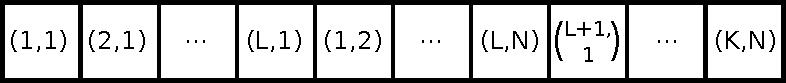
\includegraphics[width=\textwidth]{row_major_split.pdf}
	\caption{Row-major, shallow-vectorized data ordering}
	\label{F:row_major_split}
    \end{subfigure}
    \\
    \\
    \\
    \\
    \begin{subfigure}[t]{\textwidth}
	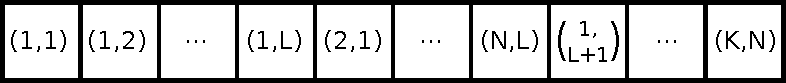
\includegraphics[width=\textwidth]{column_major_split.pdf}
	\caption{Column-major, deep-vectorized data ordering}
	\label{F:column_major_split}
    \end{subfigure}
  \end{minipage}
  \caption{Vectorized data ordering patterns}
  \label{F:vector_data}
\end{figure}

Finally,~\cref{F:vector_data} shows a vectorized data-ordering that improves the caching patterns of a shallow, ``C''-ordered SIMD vectorization on the CPU (\cref{F:row_major_split}) and a deep, ``F''-ordered SIMT vectorization on the GPU (\cref{F:column_major_split}).
This is accomplished by splitting the slower-varying axis of the data array---columns for ``C''-ordering, and rows for ``F''-ordering---into chunks of size $N_v$ (the SIMD vector-width, or SIMT warp-size) and laying these data out contiguously in memory.
For example, using the shallow-vectorized ``C''-ordering pictured in~\cref{F:row_major_split}, the concentration of species $j$ for states $i\ldots i+N_v$, $[C]_{i, j} \ldots [C]_{i + N_v, j}$, are contiguous in memory and are followed by the concentration of species $j + 1$ for the same states, $[C]_{i, j + 1} \ldots [C]_{i + N_v, j + 1}$.
This pattern, similar to OpenCL's native vector data-types---e.g., \texttt{double\num{8}} which treats \num{8} contiguous double precision floating point numbers as a single vector datum---ensures that any SIMD operation occurs on data that is contiguous in memory, greatly improving caching and SIMD-throughput.
Conversely, the data-ordering in~\cref{F:column_major_split} is designed to enable coalesced memory accesses for ``F''-ordered, deep-SIMT vectorization on the GPU.
The effects of these various data-ordering and vectorization patterns on performance will be studied in~\cref{S:results}.

\subsection{thermochemical Source-Terms and Jacobian}
This new version of \texttt{pyJac} is capable of evaluating the thermochemical source-terms for using both the constant-pressure (\conp/) or constant-volume (\conv/) assumption\footnote{Note: in this context, the ``constant-pressure'' and ``constant-volume'' assumptions refer to evaluation within a reaction sub-step in the operator splitting scheme, rather than a general constant-pressure or constant-volume reactive-flow simulation.}
In this section, we will only outline a brief summary of the system evaluated by \texttt{pyJac}; the interested reader is referred to the supplemental material for the complete derivations.


The thermochemical state vector derivation consists of the temperature, a non-constant thermodynamic state parameter (volume or pressure for \conp/ and \conv/, respectively), and the number of moles of all species except the last species in the chemical model which is typically taken to be the bath-gas (e.g., \ce{N2}):
\loadeq{state}
where $T$ is the temperature, $V$ and $P$ the volume and pressure, respectively, and $n_j$ the number of moles of the $j$th species in the model (containing $\ns/$ total species).

This state vector---inspired by~\cite{SCHWER2002270}---has a number of features that recommend its use.
First, the state vector results in highly sparse chemical kinetic Jacobians as will be detailed in~\cref{S:sparsity}.
Second, mass is explicitly conserved in this formulation owing to the fact that the moles of the final species is calculated from the ideal gas law, and the rate of change of the final species from conservation of mass (see \cref{deriv-s:state,deriv-s:source} of the supplemental material, respectively); additionally, system is not over-constrained~\cite{HANSEN2018257} and does not require use of a more complicated differential algebraic equation solver (as compared to an ODE integrator) for integration.
Finally, the chemical kinetic Jacobian changes relatively little between the \conp/ and \conv/ forms, making maintaining the code-base much simpler.
Although most current combustion codes do not use species moles as a state variable, conversion to\slash from more common mass\slash mole-fractions and moles is straightforward, and once inside integration of an chemical kinetic initial value problem (IVP), the choice of variables no longer matters.

The evolution of the thermochemical state vector is described by a set of chemical kinetic ordinary differential equations:
\loadeq{dstate}

For both \conp/ and \conv/, the molar source-terms are~\cite{TurnsStephenR2012Aitc}:
\loadeq{dmolar}
where $\dot{\omega}_k$ is the $kth$ species' overall molar production rate:
\begin{equation}
 \dot{\omega}_{k} = \sum_{i=1}^{\nr/} \nu_{k, i} R_{i} c_{i}
\end{equation}
with $\nu_{k, i}$ the net stoichiometic coefficient of species $k$ in reaction $i$, $R_{i}$ the net rate of progress of reaction $i$ (described in~\cref{deriv-s:rop_net} of the supplemental material), and $c_{i}$ the pressure-dependent modification term, i.e., for third-body (see~\cref{deriv-s:thdbody} of the supplemental material), or falloff\slash chemically-activated reactions (\cref{deriv-s:falloff} of the same); \texttt{pyJac} is capable of evaluating all modern reaction types, e.g., P-Log and Chebyshev reactions.
In addition, $N_{reac}$ is the total number of reactions in the chemical kinetic model.

The temperature source-term~\cite{TurnsStephenR2012Aitc} is:
\loadeq{dtemp}
where $H_k$, $U_k$, $C_{p,k}$ and $C_{v, k}$ are the enthalpy, internal energy, constant-pressure specific heat and constant-volume specific heat of species $k$ in molar units respectively, while $[C]_{k}$ is the concentration, given by:
\begin{equation}
 [C]_{k} = \frac{n_{k}}{V}
\end{equation}
By differentiating the ideal gas law:
\begin{equation}
 PV = n\mathcal{R}T \;,
\end{equation}
where $\mathcal{R}$ is the ideal gas-constant in molar units, the volume and pressure source-terms can be found (where $W_k$ and $W_{\ns/}$ are the molecular weights of species $k$ and $\ns/$, respectively):
\loadeq{dparam}

The Jacobian entries computed by \texttt{pyJac} are arranged such that entry ($i$, $j$) corresponds to the partial derivative of the $i$th source-term in~\cref{e:source_terms} by the $j$th state variable in~\cref{e:state}:
\loadeq{jacgeneral}

\delete{The derivative of the temperature source-term with respect to itself is:\ldots}
\add{The complete derivation of the Jacobian for \texttt{pyJac} is attached as supplemental material for the interested reader.}

\subsection{Code Generation and Testing Infrastructure}
\label{s:unittest}
Code generation is enabled by the python package \texttt{loo.py}~\cite{kloeckner_loopy_2014}, which translates pseudo-code and data to OpenCL\slash C-code.
As the name implies, \texttt{loo.py} generates code based on for-loops; this differs from the previous version of \texttt{pyJac}~\cite{pyjac16} which generates static code (i.e., fully unrolled loops, with thermodynamic\slash reaction parameters written directly in code rather than stored in arrays).
In our previous work~\cite{Niemeyer:2016aa}, this static code generation caused some issues with large file sizes, long compilation times and even occasionally breaking the \texttt{gcc} and \texttt{nvcc} compilers (the latter issue necessitated breaking the Jacobian\slash source-term evaluations into separate files).
The implications of this change will be studied in~\cref{S:jacobian_results}, where the performance of the new version of~\texttt{pyJac} will be compared to the previous version.

In addition, \texttt{loo.py} allows the user to more easily make changes to the structure of the generated program, e.g., the data ordering, vectorization, and threading patterns, as well as switching the target-language for code-generation (and simpler extension to additional languages, e.g., CUDA).
Further, \texttt{loo.py} can execute developed subroutines from python (natively for C-code, or via \texttt{PyOpenCL}~\cite{kloeckner_pycuda_2012} for OpenCL-code), enabling unit-testing\slash validation for each component of the Jacobian or source-terms.
The source-terms and sub-components thereof (e.g., rates of progress, pressure-modification terms, etc.) are directly compared to Cantera~\cite{Cantera}, while the automatic differentiation code Adept~\cite{hogan2014fast,adept-v11} is used to obtain reference answers for Jacobian sub-components.
The Portable OpenCL (POCL) implementation~\cite{poclIJPP} and OpenMP~\cite{dagum1998openmp} are used to run OpenCL and C unit-testing, respectively, on the continuous integration framework Travis CI~\cite{travis:2018}.
Validation of the complete (as opposed to the sub-component testing discussed here) generated source-terms and Jacobian codes will be discussed in detail in~\cref{s:validation}.


\section{Results and Discussion}
\subsection{Testing platforms}
\label{s:test_platforms}

\begin{table}[htb]
\centering
\begin{tabular}{@{}l l l@{}}
\toprule
CPU Model        & Xeon X5650      & E5-2690 V3     \\
\midrule
Instruction Set  & SSE4.2 	   & AVX2 	    \\
Vector Width     & \SI{2}{\doubles}&\SI{4}{\doubles}\\
Cores            & $2 \times 6$    & $2 \times 12$  \\
Identifier       & \sse/ 	   & \avx/  	    \\
OpenCL Version   & \num{1.2}       & \num{1.2}      \\
\bottomrule
\end{tabular}
\caption{The Intel CPU configurations used in this study.
	 The vector-width reported in this table is reported in (ideal) number of double operations per SIMD instruction, as this will be used in measuring SIMD efficiency; for reference, the vector-width in bits of the \sse/ and \avx/ machines are \SI{128}{\bit} and \SI{256}{\bit}, respectively.
	 The identifier field will be used as a shorthand descriptor in the performance plots to quickly identify the CPU type.}
\label{t:cpus}
\end{table}

The performance and validation studies for this work were run on a variety of CPU and GPU platforms.
\Cref{t:cpus} shows the number of cores, vector instruction set and model of the CPUs used in this work; each CPU had both \texttt{v16.1.1} of the Intel OpenCL runtime~\cite{intelopencl:2018} and \texttt{v1.0} of the POCL~\cite{poclIJPP} runtime installed, each enabling OpenCL \texttt{v1.2} execution.
Additionally, \texttt{v5.0} of the LLVM\slash\texttt{clang}~\cite{Lattner:2004:LCF:977395.977673} compiler chain was installed on all machines to enable use of POCL.
\Cref{t:gpus} lists the model, number of CUDA cores and Nvidia driver of each of the GPUs used in this work.
Nvidia's OpenCL runtime is bundled with the Nvidia driver~\cite{Nvidia:2018}, hence the driver version is used to specify the OpenCL runtime version.

\begin{table}[htb]
\centering
\begin{tabular}{@{}l l l l l@{}}
\toprule
Nvidia Model   & Tesla C2075    & Tesla K40m    \\
\midrule
Driver Version & \num{384.81}   & \num{387.26}  \\
CUDA Cores     & \num{448}      & \num{2880}    \\
Identifier     & \gpuold/ 	& \gpunew/	\\
OpenCL Version & \num{1.1}	& \num{1.2}	\\
\addtocounter{footnote}{1}
Memory\footnotemark[\thefootnote] & \SI{6}{\giga\byte} & \SI{12}{\giga\byte} \\
\bottomrule
\end{tabular}
\caption{The Nvidia GPU configurations used in this study.  Nvidia's OpenCL runtime is provided with the graphics driver, rather than any specific version of CUDA.
Again, the identifier field will be used as a shorthand descriptor during analysis of the performance results.
}
\label{t:gpus}
\end{table}
\footnotetext{Due to a driver implementation issue~\cite{Nvidia_memory}, the total memory used on the \gpuold/ and \gpunew/ GPUs were to limited to \SI{4}{\giga\byte} and \SI{10}{\giga\byte}, respectively.\addtocounter{footnote}{1}}


\Cref{t:platforms} lists the platforms and vectorization\slash execution patterns that they are capable of running.
The Intel and Nvidia OpenCL runtimes lack implementations of atomic operations on double precision variables; these are currently necessary for \texttt{pyJac} to run deep-vectorized code.
On the other hand, POCL is an open source OpenCL runtime that works on all CPU types tested in this work, and does implement these atomic operations.
However, POCL's implicit vectorization module---which utilizes the LLVM compiler~\cite{Lattner:2004:LCF:977395.977673} to translate OpenCL code to vectorized machine code---typically fails to achieve much speedup, if any.
Thus POCL is a particularly useful tool for validation, but not necessarily for performance studies.
This discussion will be expanded upon in~\cref{S:future} to highlight future directions.

\begin{table}[htb]
\centering
\begin{tabular}{@{}l c c c@{}}
\toprule
Platform & Parallel & Shallow Vectorization & Deep Vectorization \\
\midrule
OpenMP & X & -- & -- \\
POCL OpenCL & X & X & X \\
Intel OpenCL & X & X & -- \\
Nvidia OpenCL & -- & X & -- \\
\bottomrule
\end{tabular}
\caption{The various platforms used in this study and the execution \slash vectorization patterns that they are capable of running}
\label{t:platforms}
\end{table}

Finally, \cref{t:models} displays the chemical kinetic models used in this work, as well as number of partially stirred reaction conditions (PaSR) used in the condition database for each.
Creation of the PaSR databases is described in detail in our previous works~\cite{CurtisGPU:2017,Niemeyer:2016aa}.

\begin{table}[htb]
\centering
\begin{tabular}{@{}l c c @{}}
\toprule
Model &  Number of Conditions & Reference \\
\midrule
\ce{H2}\slash\ce{CO} & \num{900900} & \cite{Burke:2011fh} \\
GRI-Mech.~3.0         & \num{450900} & \cite{smith_gri-mech_30} \\
USC-Mech II           & \num{91800}  & \cite{Wang:2007} \\
\ce{iC5H11OH}         & \num{450900} & \cite{Sarathy:2013jr} \\
\bottomrule
\end{tabular}
\caption{The chemical kinetic models used in this study and number of conditions in the partially stirred reactor database for each.}
\label{t:models}
\end{table}


\subsection{Source-term validation}
\label{s:validation}
The reaction rates of progress (ROP), species and temperature rates in this study are validated by comparison with Cantera~\cite{Cantera}.
However special care must be taken due floating point arithmetic issues.

For a direct comparison, a relative error norm of a quantity $X_{ij}$ over all states $j$, and reactions (or species) $i$ was computed using the $L^{\infty}$ norm:
\begin{equation}
E_{X} = \left\lVert \frac{\left\lvert X_{ij,\text{CT}} - X_{ij}\right\rvert}{\num{e-10} + \num{e-6} * \left\lvert X_{ij,\text{CT}} \right\rvert} \right\rVert_{i,j,\infty}
\label{e:rel_err}
\end{equation}
where the \text{CT} subscript indicates values from Cantera~\cite{Cantera}

However, in computing the net ROP of reaction $i$ for state $j$ from the forward and reverse ROP: $R_{ij} = R_{ij}^{\prime} - R_{ij}^{\prime\prime}$, accuracy can easily be lost as the net ROP may be---particularly near chemical equilibrium---many orders of magnitude smaller than the forward and\slash or reverse rates.
To quantify this phenomena, the error in forward ROP is first defined as:
\begin{equation}
\varepsilon^{\prime}_{ij} = \left\lvert R_{ij}^{\prime} - R_{ij,\text{CT}}^{\prime} \right\rvert
\end{equation}
while the error in reverse ROP, $\varepsilon^{\prime\prime}_{ij}$, can be defined analogously.
Finally, for the reaction $i^{*}$ and the state $j^{*}$ that result in the largest error in net ROP, i.e. $E_{R}$, an estimate of the error attributable to floating point error accumulation from the forward and reverse ROPs can be obtained as:
\begin{equation}
E_{\varepsilon} = \frac{\max(\varepsilon^{\prime}_{i^{*}j^{*}}\text{, }\varepsilon^{\prime\prime}_{i^{*}j^{*}})}{\num{e-10} + \num{e-6} * \left\lvert R_{i^{*}j^{*},\text{CT}} \right\rvert}
\end{equation}
This estimate allows for direct comparison of the error in forward or reverse ROPs to the value of the net ROP itself, if they are of similar magnitude the error in net ROP will be large.

\begin{table}[htbp]
\sisetup{retain-zero-exponent=true}
\centering
\begin{tabular}{@{}l S[table-format=1.2e1] S[table-format=1.2e1] S[table-format=1.2e1] S[table-format=1.2e1]@{}}
\toprule
\multicolumn{1}{l}{Model} & \multicolumn{1}{l}{\ce{H2}\slash\ce{CO}} & \multicolumn{1}{l}{GRI-Mech.~3.0} & \multicolumn{1}{l}{USC-Mech II} & \multicolumn{1}{l}{\ce{iC5H11OH}} \\
\midrule
\multicolumn{1}{c}{$E_{R^{\prime}}$}                    & 1.56e-8 & 2.95e-8 & 9.42e-8 & 4.86e-4 \\
\multicolumn{1}{c}{$E_{R^{\prime\prime}}$}              & 6.92e-8 & 6.53e-8 & 1.20e-7 & 5.07e-4 \\
\multicolumn{1}{c}{$E_{R}$}                             & 1.49e1  & 1.11e0  & 2.80e0  & 4.82e-1 \\
\multicolumn{1}{c}{$E_{\varepsilon}$}                   & 1.48e1  & 1.13e0  & 2.93e0  & 5.03e-1 \\
\multicolumn{1}{c}{$E_{\frac{\text{d} n}{\text{d} t}}$} & 2.53e1  & 2.60e0  & 7.62e0  & 1.58e1 \\
\multicolumn{1}{c}{$E_{\frac{\text{d} T}{\text{d} t}}$} & 3.94e5  & 3.35e8  & 3.95e6  & 7.11e7 \\
\multicolumn{1}{c}{$E_{\frac{\text{d} S}{\text{d} t}}$} & 3.52e12 & 3.46e12 & 3.44e12 & 3.38e12 \\
\bottomrule
\end{tabular}
\caption{Summary of rate of progress, species, temperature and thermodynamic state-parameter rate correctness.
Error statistics are based on the infinity-norm of the relative error detailed in~\cref{e:rel_err} for each quantity.
The ``S'' in $E_{\frac{\text{d} S}{\text{d} t}}$ refers to the thermodynamic state parameter, either $V$ or $P$ for \conp/ and \conv/, respectively.
}
\label{T:source_error}
\end{table}

In Table~\ref{T:source_error}, the results of this code's source-term evaluations are compared to Cantera~\cite{Cantera} on the library of PaSR conditions (\cref{t:models}).
Very close agreement is observed for the forward and reverse ROPs for all models, however the error norm is \textasciitilde\numrange{3}{4} orders of magnitude larger for the isopentanol model.
This results from differences in evaluation of P-Log reactions between \texttt{pyJac} and Cantera; namely \texttt{pyJac} computes the logarithm of the upper and lower reaction Arrhenius rates (see supplemental~\cref{deriv-s:pdep}) analytically while Cantera evaluates this term numerically.
If the error from P-Log reactions are not considered in~\cref{e:rel_err}, the errors for the forward and reverse ROPs fall to \num{5.44e-08} and \num{1.59e-07}, respectively.
We note that this discrepancy does not imply any incorrectness in either \texttt{pyJac} or Cantera---in fact, the error is still well within the proscribed tolerances in~\cref{e:rel_err}---but merely emphasizes the effect small code-changes can have on the accumulation of floating point errors.

This point is further underscored by the error in the net ROP, which is \textasciitilde\numrange{3}{9} orders of magnitude (or \numrange{7}{9} orders of magnitude for the P-Log excluded error) larger than the error in either the forward or reverse ROP.
In~\cref{T:source_error}, it is seen that $E_{\varepsilon}$ is very similar in magnitude to $E_R$ in all cases, indicating that this large increase in error is caused by the accumulation of floating point error from the forward and reverse ROPs, as previously discussed.
The molar species production rate error norm is similar in magnitude to that of the net ROP, however the temperature and state-parameter rate errors again increase as the error in net species production rates is amplified by multiplication with thermodynamic properties.
Again, we note that the above discussion does not imply that discrepancies in computation of the net ROP will cause large error in chemical kinetic integration---either in this code or Cantera~\cite{Cantera}---as this loss of accuracy only occurs when the forward and reverse ROPs are nearly equal, implying the reaction is in near-equilibrium.

\subsection{Jacobian validation}
\label{S:jac_valid}

As in our previous work~\cite{Niemeyer:2016aa}, the correctness of the Jacobian was determined by comparison to the Jacobian obtained by automatic differentiation of the source-terms kernel generated by \texttt{pyJac} via the \texttt{Adept} software library~\cite{adept-v11,hogan2014fast}.
The reasons for this choice are explained fully in~\cite{Niemeyer:2016aa}, but broadly speaking automatic differentiation provides relatively fast, highly accurate Jacobian matrix evaluation with minimal additional programming effort.
The discrepancy between the analytical and automatic differentiated Jacobians for thermochemical state $k$, denoted by $\mathcal{J}_k$ and $\hat{\mathcal{J}}_k$ respectively, is determined by the relative error Frobenius norm over all Jacobian indices $i, j$:
\begin{equation}
 \label{e:jac_error_base}
 E_{\text{rel}, k} = \left\lVert \frac{\hat{\mathcal{J}}_{ijk} - \mathcal{J}_{ijk}}{\hat{\mathcal{J}}_{ijk}} \right\rVert_{i,j,F}
\end{equation}

To avoid large relative errors of very small nonzero Jacobian elements due to accumulation of floating point error, the Frobenius norm of the automatically differentiated Jacobian is calculated over all thermochemical states $k$:
\begin{equation}
 \label{e:thresh}
 \mathcal{T} = \left\lVert \mathcal{\hat{J}} \right\rVert_{k, F}
\end{equation}
The error statistics reported in this section are then based only on matrix elements where $\mathcal{J}_{ijk} \ge \frac{\mathcal{T}}{\mathcal{C}}$, where $\mathcal{C}$ is the threshold parameter; this filtered form of~\cref{e:jac_error_base} is denoted $E_{\mathcal{C},k}$.
Finally, the Frobenius norm is calculated over all the states in the PaSR thermochemical condition database:
\begin{equation}
 \label{e:thresholded_error}
 E_{\mathcal{C}} = \left\lVert E_{\mathcal{C},k} \right\rVert_{k, F}
\end{equation}

It is noted that this error norm is quite different from the relative error Frobenius norm suggested by Anderson et al.~\cite{Anderson:1999aa} for quantifying the error of matrices in LAPACK:
\begin{align}
 \label{e:error_lapack}
 \lhs{lapack}{E_{\mathcal{L}, k}} &=  \rhs{lapack}{\frac{\left\lVert \hat{\mathcal{J}}_{ijk} - \mathcal{J}_{ijk} \right\rVert_{i,j,F}}{\left\lVert \hat{\mathcal{J}}_{ijk} \right\rVert_{i,j,F}}} \nonumber \\
 \lhs{lapack}{E_{\mathcal{L}}} &= \rhs{lapack}{\left\lVert  E_{\mathcal{L}, k} \right\rVert_{k, F}}[c]
\end{align}
In our experience, the LAPACK error norm is often dominated by the accuracy of the larger elements in the Jacobian, while the filtered error norm is useful for identifying errors in both large and small Jacobian entries.
Further, with a tunable threshold parameter, $\mathcal{C}$, the error of different ranges of of element sizes can be assessed, and the effects of floating point error can be isolated.
For reference, both our own error norm and the LAPACK error norm will be reported.

\begin{table}[htbp]
\sisetup{retain-zero-exponent=true}
\centering
\begin{tabular}{@{}l S[table-format=.0] S[table-format=1.3e1] S[table-format=1.3e1] S[table-format=1.3e1] S[table-format=1.3e1] @{}}
\toprule
Model                 & \multicolumn{1}{c}{$E_{\mathcal{L}}$} & \multicolumn{1}{c}{$\bar{\mathcal{T}}$} & \multicolumn{1}{c}{$E_{\mathcal{C} = 10^{20}}$}   & \multicolumn{1}{c}{$E_{\mathcal{C} = 10^{15}}$} \\
\midrule
\ce{H2}\slash \ce{CO} & \num{1.862e-14}      & \num{6.431e+18}      & \num{1.741e+0}  & \num{4.508e-5} \\
GRI-Mech 3.0          & \num{1.567e-14}      & \num{7.783e+19}      & \num{3.842e-7}  & \num{3.687e-7} \\
USC-Mech II           & \num{1.137e-14}      & \num{2.830e+21}      & \num{1.199e-2}  & \num{1.983e-7} \\
\ce{iC5H11OH}         & \num{1.227e-10}      & \num{2.733e+26}      & \num{1.363e-3}  & \num{2.764e-5} \\
\bottomrule
\end{tabular}
\caption{Summary of Jacobian matrix validation results.
The reported error statistics are the maximum filtered relative error $E_\mathcal{C}$ and LAPACK error $E_{\mathcal{L}}$ over all test platforms, vectorization patterns (\cref{t:platforms}),  \conp/\slash \conv/ and sparse\slash dense Jacobians.
It is noted that the Frobenius norm described in~\cref{e:thresh} varies slightly between the \conp/ and \conv/ cases; the reported $\bar{\mathcal{T}}$ is the average of the two, however the appropriate value was used during calculations of the error statistics.
}
\label{T:error}
\end{table}

\Cref{T:error} reports the maximum $E_{\mathcal{C}}$ and $E_{\mathcal{L}}$ values over all test platforms\slash vectorization patterns (see~\cref{t:platforms}), sparse\slash dense (see~\cref{S:sparsity}) and \conp/\slash\conv/ Jacobians.
The most stringent filtered error norm ($\mathcal{C} = 10^{20}$) ranges from \numrange[retain-zero-exponent=true]{e-7}{e0}; the largest error is for the \ce{H2}\slash\ce{CO} model.
For this model, $\mathcal{T}$  is smaller than the tolerance of \num{e20}, and hence the error norm considers Jacobian entries smaller than $\mathcal{O}(1)$.
It is noted that for GRI-Mech 3.0, which has a $\mathcal{T}$ roughly an order of magnitude larger, the stringent error norm is significantly smaller: $\mathcal{O}(\num{e-7})$.
Given the intricacy of floating point error evaluation, the use of different languages and OpenCL platforms (the effect of these differences will be explored in \cref{A:per_platform}), and for the general complexity of \texttt{pyJac} it would be exceedingly difficult to pinpoint an exact cause for this phenomenon, as was done in~\cref{s:validation}.
To ensure there is no bug or error present in the Jacobians generated by \texttt{pyJac}, a relaxed filtered error norm ($\mathcal{C} = 10^{15}$) is also presented for each model in~\cref{T:error}.
This relaxed norm is smaller by \numrange{2}{5} orders of magnitude for all models---except GRI-Mech 3.0, where the stringent case has very small error as previously discussed---indicating that accuracy is higher when the smaller Jacobian entries are excluded; this suggests floating point error accumulation is the primary driver of the stringent filtered error norm.

The relative LAPACK error norm---ranging from \textasciitilde\numrange{e-10}{e-14}---re-enforces this finding, as it indicates roughly \numrange{10}{14} digits of accuracy~\cite{Anderson:1999aa}.
The \ce{iC5H11OH} model has the largest LAPACK error norm, likely due to the presence of P-Log\slash Chebyshev reactions and associated complicated derivatives with many logarithms, exponetiations and summations.
Further, the LAPACK error norm does not correlate well with the stringent filtered error norm, e.g., USC-Mech II has the smallest LAPACK error norm (\num{1.137e-14}), but the second largest stringent filtered error norm (\num{1.119e-2}).
Conversely, the model with the largest LAPACK error norm, \ce{iC5H11OH} (with $E_{\mathcal{L}} = \num{1.227e-10}$), has the second smallest stringent filtered error norm (\num{1.363e-3}) , again suggesting that the stringent error norm is influenced by floating point error accumulation.
These findings, along with the individual unit-testing of all chemical source-terms and Jacobian sub-components described in~\cref{s:unittest}, gives high confidence in the correctness of this new version of \texttt{pyJac}.


\subsection{Sparsity patterns}
\label{S:sparsity}

In general, the Jacobian matrices generated by \texttt{pyJac} are largely sparse with non-zero entries corresponding mainly to species that participate in the same reaction (or non-default efficiency third-body species in a reaction), and mostly dense rows\slash columns corresponding to the temperature and thermodynamic state parameter.
However, the explicit-mass conservation formulation of \texttt{pyJac} can introduce additional non-zero entries in two ways.
First, if the last-species in the model (i.e., the bath-gas) participates directly in a reaction, the derivative of the forward or reverse rate of progress with respect to any other species is non-zero (see~\cref{deriv-s:dri_dnj} of the supplemental material).
Similarly, if the last-species has a third-body efficiency not equal to the default (unity), this will again force all the derivative of the pressure-modification term with respect to other species to be non-zero (see~\cref{deriv-s:dci_thd} of the same).
Either case will result in an undesirable fully dense Jacobian row for all species that have a non-zero net stoichiometic coefficient in such a reaction.

However, the current \texttt{pyJac} allows the user to simply ignore these derivatives (via a command-line switch) and avoid any adverse effects on the Jacobian sparsity.
The rationale behind this choice is that many common implicit integration techniques (e.g., CVODE~\cite{Hindmarsh:2005}) used in solution of chemical kinetic initial value problems are formulated around the assumption that the supplied Jacobian is approximate; this allows the Jacobian and its LU factorization to be reused for multiple internal integration time-steps, accelerating the solution process.
For such solvers, there is no need for the exact form of the Jacobian and the so-called ``approximate'' form is preferable.
\add{Though this might be used as a crude form of preconditioning for such solvers, the primary purpose is merely to increase the resulting sparsity of the Jacobian; the reader is directed to~\cite{MCNENLY2015581} for a more thorough discussion of preconditioners.}
Hence, in this section we will detail the sparsity of both forms of the Jacobian for the chemical models tested.

In~\cref{F:jac_sparsity}, a graphical representation of the sparsity pattern for GRI-Mech 3.0 is displayed.
In particular we note that~\cref{F:jac_sparse_approx} is has several rows that are no longer fully-dense, as result of its approximate form; these rows correspond to species directly interacting with \ce{N2}, largely in GRI-Mech 3.0's nitrogen chemistry reactions.
\cref{T:jac_sparsity} shows the density of the exact and approximate Jacobians for all chemical kinetic models tested in this work.
The smallest model, \ce{H2}\slash\ce{CO} is very dense with \SI{71.4}{\percent} of the exact Jacobian entries non-zero, however this drops to \SI{56.7}{\percent} for GRI-Mech 3.0, and continues to decrease to \SI{28.2}{\percent} for USC-Mech II and just \SI{11.5}{\percent} for the isopentanol model.
The approximate Jacobian assumption drops the density of Jacobian by \textasciitilde\SIrange{3}{7}{\percent} for all models.

\begin{figure}[htb]
  \centering
  \begin{subfigure}[t]{0.48\linewidth}
      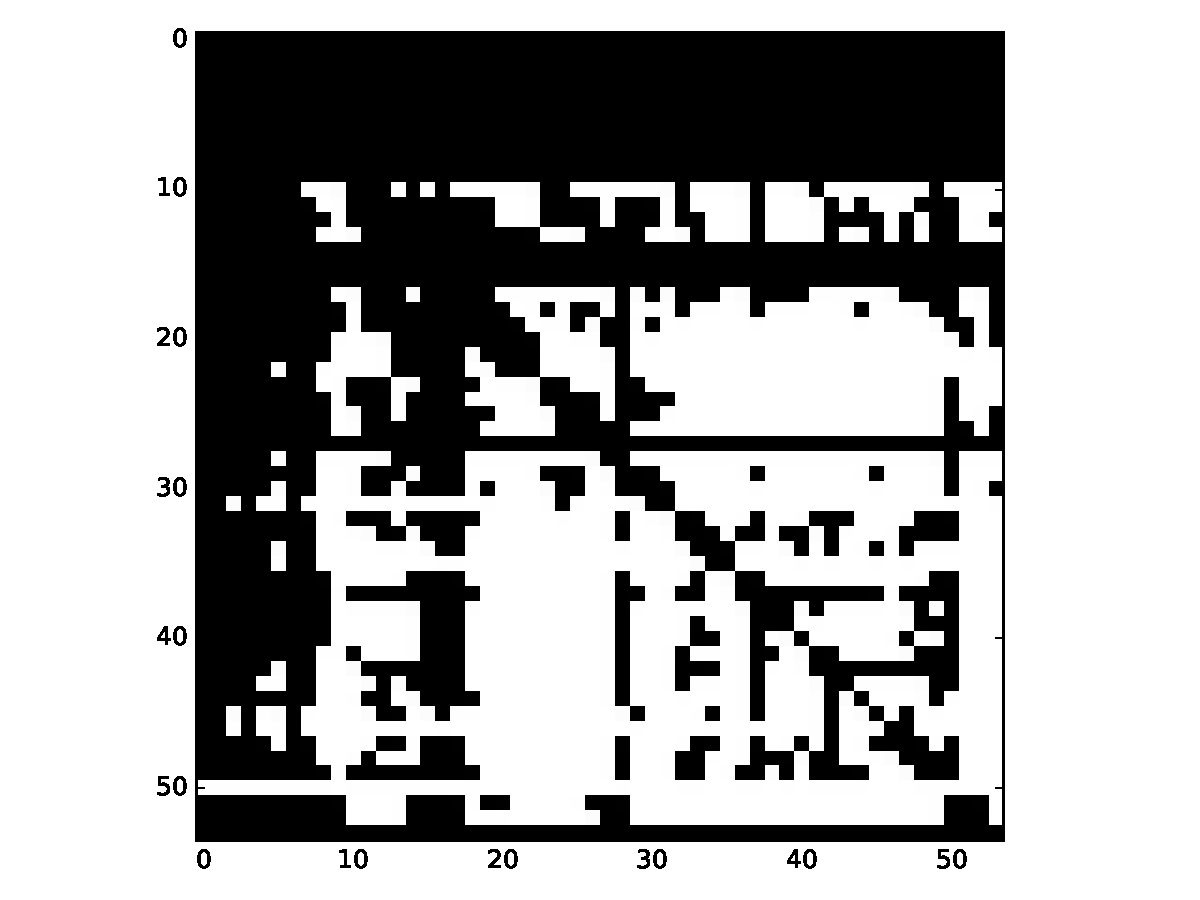
\includegraphics[width=\textwidth]{ch4_sparsity_exact.pdf}
      \caption{The ``exact'' Jacobian.}
      \label{F:jac_sparse_exact}
  \end{subfigure}
  \hfill
  \begin{subfigure}[t]{0.48\linewidth}
      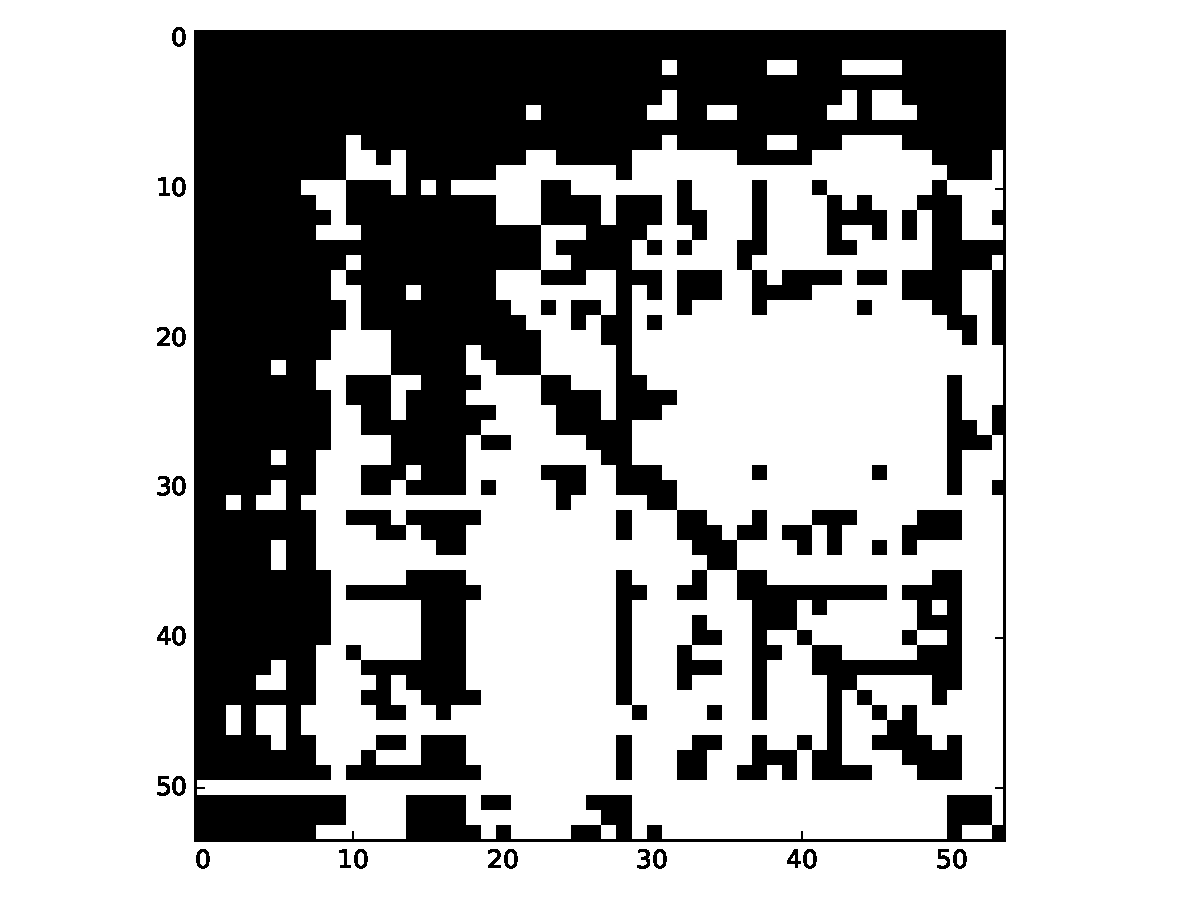
\includegraphics[width=\textwidth]{ch4_sparsity_approximate.pdf}
      \caption{The ``approximate'' Jacobian.}
      \label{F:jac_sparse_approx}
  \end{subfigure}
  \caption{A graphical representation of the sparsity pattern of the chemical kinetic Jacobian generated by \texttt{pyJac} for GRI-Mech 3.0.
	   Black squares indicate a non-zero Jacobian entry, while white square correspond to an empty entry.
	   The numbers indicate the index of the entry in the state vector.}
  \label{F:jac_sparsity}
\end{figure}

Currently, \texttt{pyJac} can utilize two common sparse matrix storage formats~\cite{netlib_templates}, compressed row\slash column storage (CRS\slash CCS), used for ``C'' and ``F''-ordered data respectively.
For convenience we will outline only the CRS format but the CCS format is very similar~\cite{netlib_templates}.
An $N\times N$ CRS matrix is composed of three vectors, a value vector of length $NNZ$---the number of non-zero elements in the Jacobian---which stores the elements of the Jacobian, a row pointer vector---of length $N$---which stores the locations in the value vector that begin a row, and a column index vector---of length $NNZ$---which stores the column indices of the elements in the value vector.

\begin{table}[tbp]
\centering
\begin{tabular}{@{}l S[table-format=2.1] S[table-format=2.1]@{}}
\toprule
Model                 & \multicolumn{1}{c}{Exact Jacobian Density} & \multicolumn{1}{c}{Approximate Jacobian Density} \\
\midrule
\ce{H2}\slash \ce{CO} & \SI{71.4}{\percent} & \SI{68.4}{\percent} \\
GRI-Mech 3.0          & \SI{56.7}{\percent} & \SI{49.8}{\percent} \\
USC-Mech II           & \SI{28.2}{\percent} & \SI{26.4}{\percent} \\
\ce{iC5H11OH}         & \SI{11.5}{\percent} & \SI{7.98}{\percent} \\
\bottomrule
\end{tabular}
\caption{The density of the exact and approximate Jacobians generated by \texttt{pyJac} for the various models studied.}
\label{T:jac_sparsity}
\end{table}

The Jacobian access pattern used by \texttt{pyJac} is fairly irregular; for simplicity we will only discuss looping-structure of species derivatives calculations as these form the bulk of the computation, and have the most challenging Jacobian access patterns.
In general, an outer loop iterates over all reactions of a certain type (e.g., falloff reactions) and calculates the relevant Jacobian subproducts---independent of any particular species---for the reaction (e.g., the derivative of the falloff pressure modification term).
Two inner loops then iterate over the species in a reaction, updating the Jacobian entries for these species as appropriate.
This pattern leads to fairly easily vectorizable code, and efficient Jacobian evaluation as the bulk of the computation is dependent only on the reaction in question, as discussed in our previous work~\cite{Niemeyer:2016aa}.
Generally, this means that a lookup operation is required to find the sparse Jacobian index for any pair of state variables; in some cases this can be avoided, e.g., the rows corresponding to derivatives of the temperature and thermodynamic state parameter source-terms are fully dense in \texttt{pyJac}, and hence no lookup is necessary.
This lookup operation is currently implemented as a simple for-loop, e.g., for a sparse lookup of a pair of indices $(i, j)$ in a CRS matrix, the lookup function searches the column index vector between the values $\texttt{row\_pointer}[i] \ldots \texttt{row\_pointer}[i + 1]$ for $j$, and returns the offset from $\texttt{row\_pointer}[i]$ (or $\num{-1}$ if not found).
As will be explored in~\cref{S:jacobian_results}, this slows down sparse Jacobian evaluation, and might be improved---at the cost of increased constant data usage, a limitation for OpenCL---by a static mapping of the full Jacobian indices to the sparse index (or some null value if the entry is empty).
Additionally, this might be an excellent usage of OpenCL's Image memory type (similar to texture memory in CUDA terminology) and both of these sparse indexing techniques merit future investigation.


\subsection{Performance}
\label{S:results}
The performance studies in this work were run on the platforms listed in~\cref{t:cpus,t:gpus}.
Run times in each case were averaged over ten runs, each using the same set of PaSR conditions utilized in validation.
The OpenMP Jacobian\slash source-term kernels, as well as the OpenMP\slash OpenCL wrapping code---responsible for initializing\slash transferring memory, reading input, etc.---was compiled with \texttt{gcc v5.4.0} on the \avx/\slash\gpunew/ platforms, and \texttt{gcc v4.8.5} on the \sse/\slash\gpuold/ machines.
The optimization level ``\texttt{-O3 -mtune=native}'' was used, and no ``fast-math'' OpenCL optimizations were enabled.
Additionally, the exact form of the Jacobian (as opposed the the ``approximate'' form discussed in~\cref{S:sparsity}) was used in all cases.
Finally, unless stated otherwise: the performance results utilized a single CPU core, the \conp/ assumption, a vector-width of \num{8}\slash\num{128} and ``C''\slash ``F''-ordered data for the CPU\slash GPU cases, respectively; the run times reported are for the number of conditions specified in~\cref{T:error} and include data transfer overhead to\slash from internal buffers used in \texttt{pyJac}.
The effects of choice of vector-width, data-ordering and differences between \conp/ and \conv/ evaluations on the CPU\slash GPU will be explored in~\cref{S:source_results}, while parallel scaling for multiple CPU cores will be exampled in~\cref{S:source_results,S:jacobian_results}.

\subsubsection{Source-term evaluation}
\label{S:source_results}

\Cref{F:cpu_source} explores the performance of the source-term evaluations generated by \texttt{pyJac} on the CPU test platforms listed in~\cref{t:cpus}.
Source-term evaluations---critical in their own right for direct numerical simulations of reacting flows~\cite{Spafford:2010aa}, among other applications---also give a convenient platform to detail the effects of various code configuration options before investigating the more involved Jacobian evaluation performance.

In~\cref{F:intel_source_nonorm}, the mean run time per initial condition is shown for both the~\avx/ and~\sse/ CPUs, using both Intel OpenCL and OpenMP.
This normalization of the run time by the number of initial conditions tested is chosen to account for the varying numbers of conditions in the PaSR databases for each model (\cref{t:models}).
For both CPUs, the OpenMP implementation is the slowest over all models; interestingly the unvectorized (strictly parallel) Intel OpenCL code is slightly faster than OpenMP in all cases.
As expected, the \avx/ machine is faster than the \sse/ CPU for the strictly parallel cases, \SIrange{1.82}{2.13}{$\times$} for the unvectorized OpenCL case, and \SIrange{1.72}{1.85}{$\times$} for OpenMP.
Additionally, the shallow-vectorized OpenCL code is significantly faster than either the OpenMP or unvectorized OpenCL codes on both processors.

\begin{figure}[htbp]
   \centering
  \begin{subfigure}[t]{0.48\linewidth}
      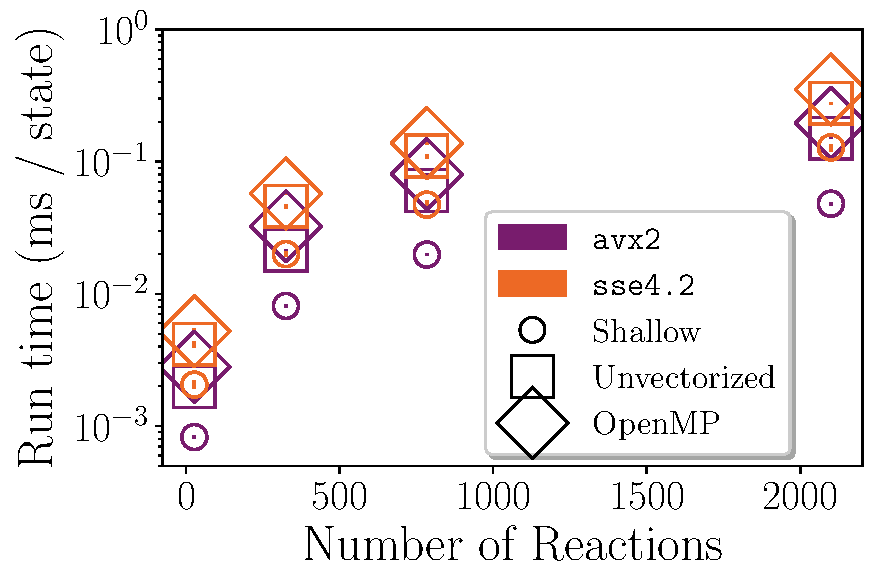
\includegraphics[width=\textwidth]{intel_source_nonorm.pdf}
      \caption{The mean run time per condition for each chemical model using the Intel OpenCL and OpenMP on both CPUs studied.}
      \label{F:intel_source_nonorm}
  \end{subfigure}
  \hfill
  \begin{subfigure}[t]{0.48\linewidth}
      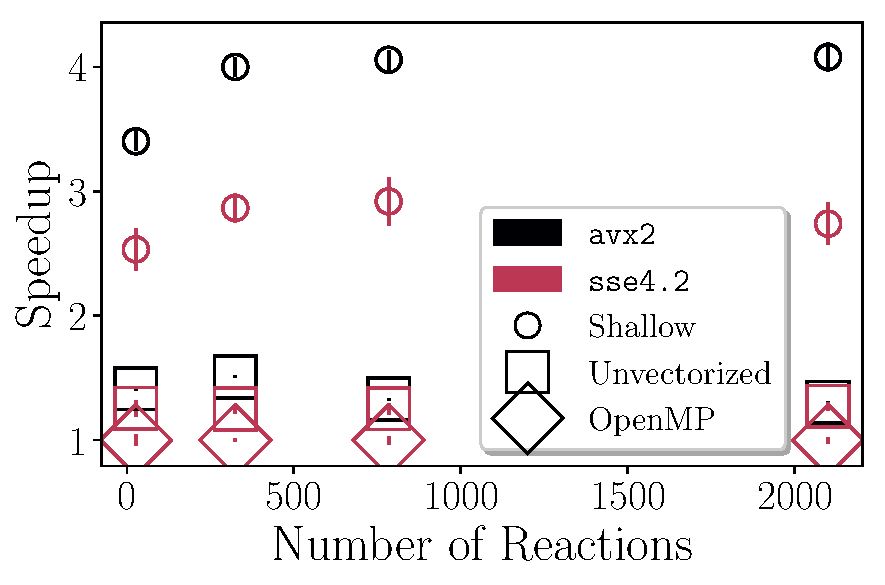
\includegraphics[width=\textwidth]{intel_source.pdf}
      \caption{The speedup achieved over the baseline OpenMP parallelization by both the unvectorized and shallow-vectorized Intel OpenCL codes; the speedup is presented on per-machine basis.}
      \label{F:intel_source}
  \end{subfigure}
  \\
  \begin{subfigure}[t]{0.48\linewidth}
      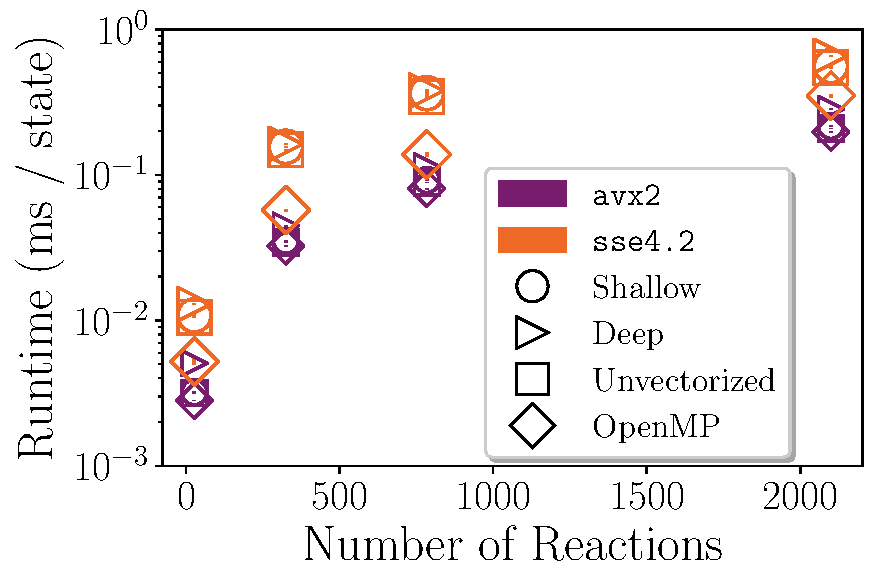
\includegraphics[width=\textwidth]{pocl_source_nonorm.pdf}
      \caption{The mean run time per condition of the Portable OpenCL runtime compared to OpenMP parallelization.}
      \label{F:pocl_source}
  \end{subfigure}
 \caption{Mean run times per condition and speedups achieved by the various CPU OpenCL runtimes compared to OpenMP parallelization for each chemical model studied. The names in the legends correspond to the identifiers listed in~\cref{t:cpus}.}
 \label{F:cpu_source}
\end{figure}

In~\cref{F:intel_source}, the extent of this speedup is detailed; we note that the speedup displayed is calculated per-machine, e.g., the \avx/ shallow-vectorized code speedup is relative to OpenMP on the same CPU such that the speedup of the shallow-vectorized OpenCL code can be readily assessed.
On both machines, the unvectorized OpenCL code is faster than the baseline parallel OpenMP code; by \SIrange{1.30}{1.51}{$\times$} on the \avx/ CPU, and \SIrange{1.25}{1.27}{$\times$} on the \sse/ machine.
Additionally, the shallow-vectorized OpenCL code is \SIrange{2.53}{2.92}{$\times$} and \SIrange{3.40}{4.08}{$\times$} faster than the OpenMP code for the \sse/ and \avx/ machines, respectively.

In contrast,~\cref{F:pocl_source} shows the mean run time per condition of deep, shallow and unvectorized OpenCL codes on the POCL runtime, as compared to OpenMP parallelization.
No speedup is achieved for either vectorization type on either CPU---\add{though we stress that Intel OpenCL runtime achieved vectorization using the same code and hardware}---indeed, the OpenMP case is faster on both CPUs.
The reasons for this lack of vectorization are quite technical,~\delete{and somewhat outside the scope of this work}however \add{personal communications~\cite{pocl_communication} with the developers of POCL revealed that in order to achieve vectorization, changes are required to both the way POCL prepares LLVM \cite{Lattner:2004:LCF:977395.977673} IR-code---specifically, to specialize boundary cases to ensure LLVM recognizes uniform vectorization loop-bounds, even if said bounds \textit{are} uniform in practice---as well as improvements to LLVM's loop-vectorizer: e.g., for proofs of a vector instruction's ability to handle all edge cases identically to the corresponding scalar instruction, handing of branches and conditionals (potentially within POCL instructions themselves), and handling of memory access\slash vector-element extraction patterns.}
As will be discussed in~\cref{S:future}, \add{it is hoped that use of explicit vector-types (to lessen demands on the LLVM-vectorization module) in combination with some of these changes might solve this issue}, but for the moment POCL is still quite useful as a validation tool.

\Cref{F:gpu_source} shows the performance of the source-term evaluation on the GPUs listed in~\cref{t:gpus}.
In~\cref{F:gpu_source_scaling}, the number of initial conditions over which the source-terms are evaluated on the \gpunew/ GPU is varied in order to determine the effect on the mean run time per condition; the run time continues to decrease until \textasciitilde\num{e4} conditions for all chemical models (except the \ce{H2}\slash\ce{CO} model, which is closer to \textasciitilde\num{3e4} conditions), at which point the GPU becomes saturated and performance levels off.
\Cref{F:gpu_source_speedup} shows the speedup in source-term evaluations that the \gpunew/ GPU achieves over the \gpuold/ GPU for the maximum number of conditions in~\cref{F:gpu_source_scaling} with two different vector-widths (a.k.a., the block size in Nvidia terminology), \num{64} and \num{128}; the fastest \gpunew/ case with a vector-width of 128 is \SIrange{1.40}{1.88}{$\times$} faster than the slowest case (\gpuold/ with a vector-width of \num{64}) depending on the chemical model in question.
Additionally,~\cref{F:gpu_source_speedup} shows that varying the vector-width has minimal effect on performance for most of the \gpunew/ and \gpuold/ cases; the GRI-Mech 3.0 and USC-Mech II models show the largest improvements with a vector-width of \num{128}, \textasciitilde\SIrange{10}{18}{\percent} for both GPUs.
This is likely caused by higher occupancy on the GPUs, however it is unclear exactly how Nvidia's OpenCL runtime balances the registers\slash warps per streaming-multiprocessor, as controls occupancy in CUDA~\cite{occupancy}; use of even larger vector-widths (i.e., \num{256}\texttt{+}) on the GPU is a topic that merits future investigation.
\begin{figure}[htbp]
   \centering
  \begin{subfigure}[t]{0.48\linewidth}
      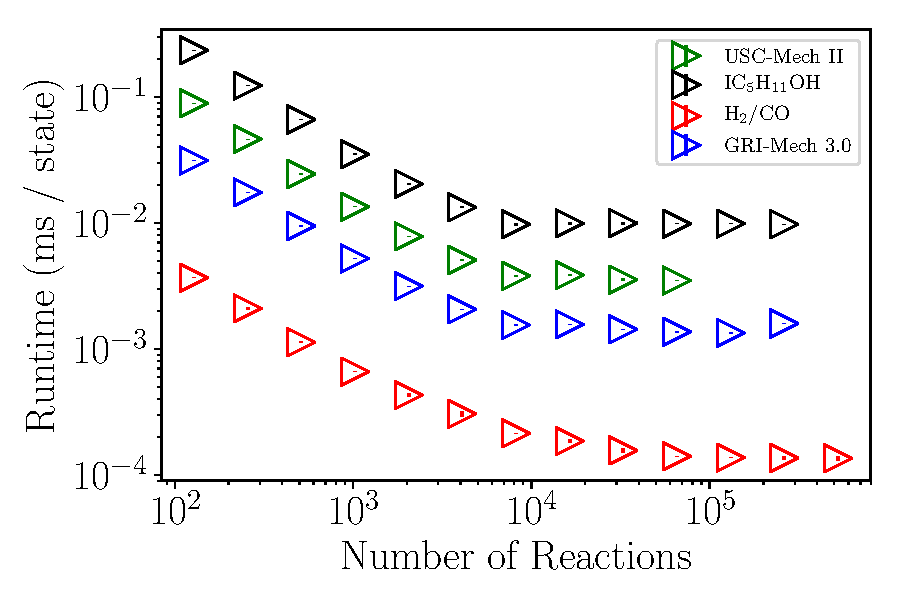
\includegraphics[width=\textwidth]{gpu_source_scaling.pdf}
      \caption{The mean run time per condition for each chemical model on the \gpunew/ GPU as a function of the number of initial conditions tested.}
      \label{F:gpu_source_scaling}
  \end{subfigure}
  \hfill
  \begin{subfigure}[t]{0.48\linewidth}
      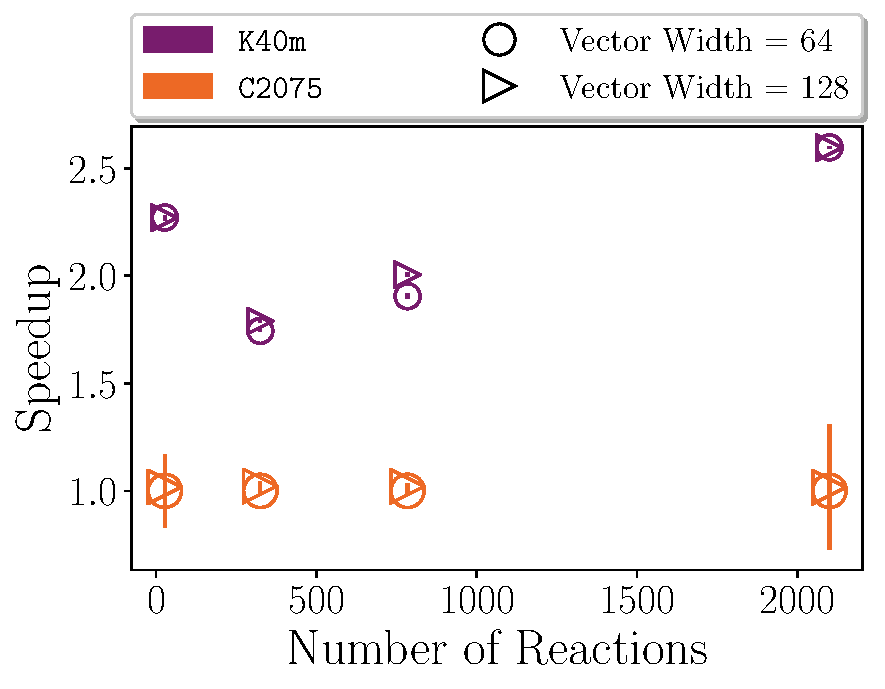
\includegraphics[width=\textwidth]{gpu_source_speedup.pdf}
      \caption{The speedup achieved on the \gpunew/ versus the \gpuold/ GPU; the names correspond to the identifiers listed in~\cref{t:gpus}}
      \label{F:gpu_source_speedup}
  \end{subfigure}
  \caption{\texttt{pyJac} source-term evaluation performance on the Nvidia GPUs}
  \label{F:gpu_source}
\end{figure}

\Cref{f:source_permutate} shows the effect of changing data-ordering patterns, the \conp/ or \conv/ formulation, and the CPU vector-width size on the performance of source-term evaluation in \texttt{pyJac}.
In~\cref{F:source_conpvsconv}, it is seen that choice of the \conp/ or \conv/ formulation has little to no effect on run time for OpenMP as well as the shallow-vectorized\slash unvectorized Intel OpenCL codes on the \avx/ machine.
Generally speaking, the difference between the \conp/ and \conv/ formulations has only a marginal effect on performance regardless of CPU\slash GPU choice.

\begin{figure}[htbp]
   \centering
  \begin{subfigure}[t]{0.48\linewidth}
      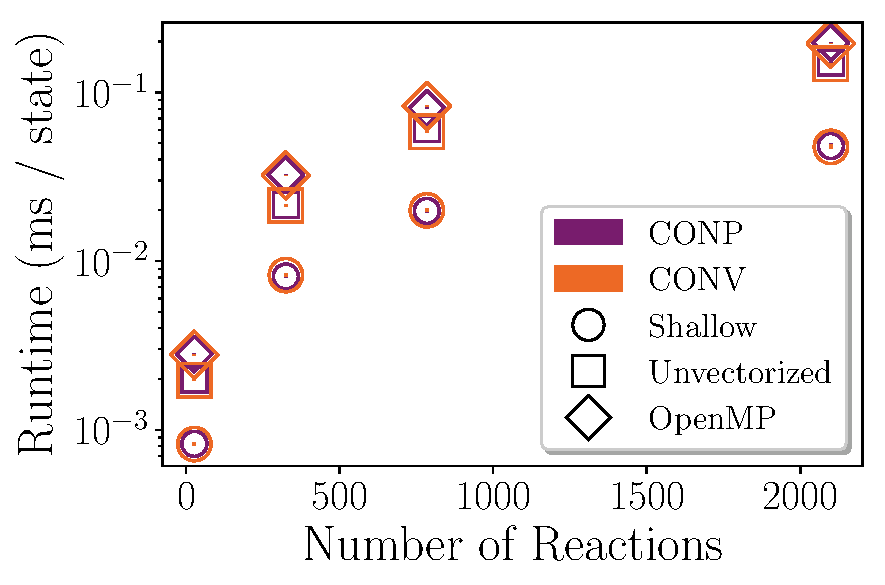
\includegraphics[width=\textwidth]{source_conpvsconv.pdf}
      \caption{The mean run time per condition for each chemical model using both the \conp/ and \conv/ formulations on Intel OpenCL and OpenMP on the \avx/ CPU.}
      \label{F:source_conpvsconv}
  \end{subfigure}
  \hfill
  \begin{subfigure}[t]{0.48\linewidth}
      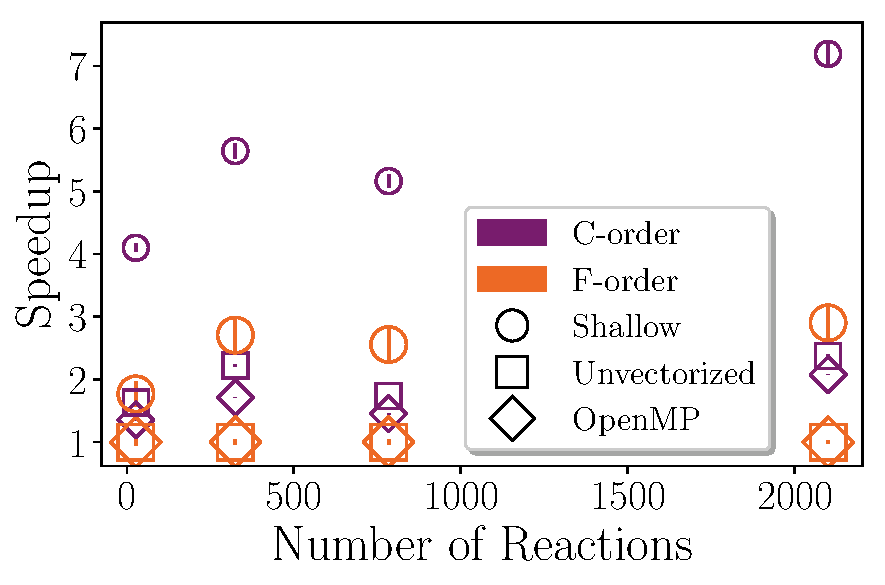
\includegraphics[width=\textwidth]{source_cvsf.pdf}
      \caption{The speedup achieved by ``C'' ordering over ``F'' ordering for Intel OpenCL and OpenMP on the \avx/ CPU.  The speedup presented is calculated per-language (OpenMP and OpenCL) to better assess the effect of the data-ordering.}
      \label{F:source_cvsf}
  \end{subfigure}
  \\
  \begin{subfigure}[t]{0.48\linewidth}
      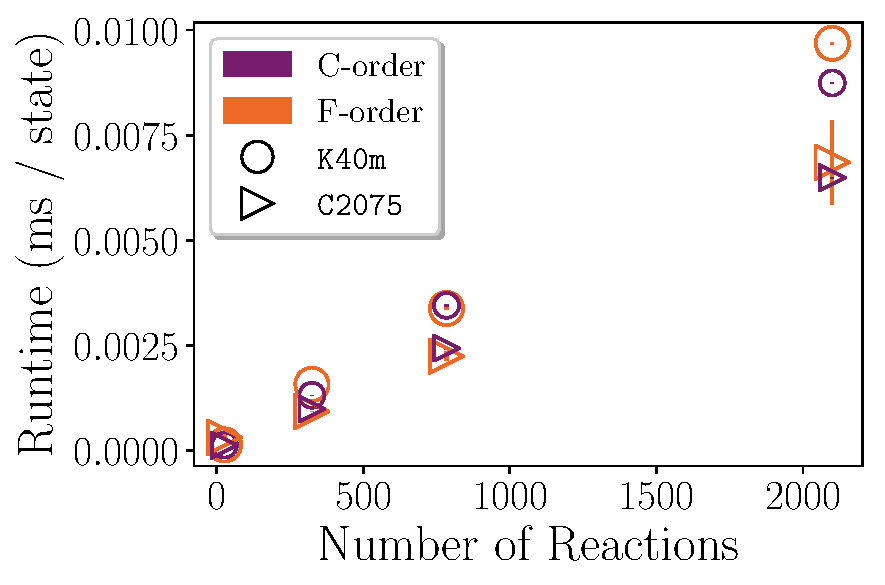
\includegraphics[width=\textwidth]{source_gpu_cvsf.pdf}
      \caption{The affect on performance of ``C'' vs ``F''-ordering for the shallow-vectorized Nvidia OpenCL code on both GPUs with a vector-width of \num{128}.}
      \label{F:source_gpu_cvsf}
  \end{subfigure}
  \hfill
  \begin{subfigure}[t]{0.48\linewidth}
      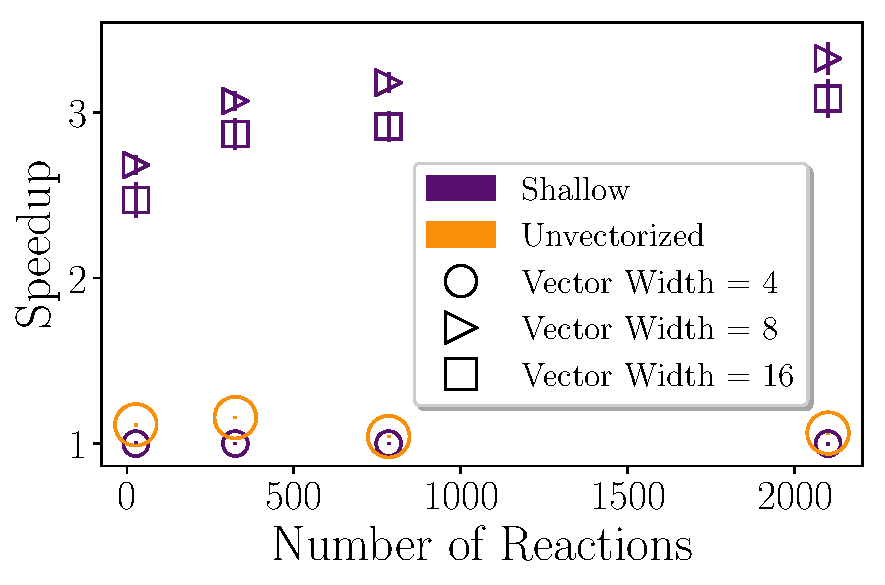
\includegraphics[width=\textwidth]{source_vector_width.pdf}
      \caption{The effect of vector-width on ``C''-ordered shallow-vectorized Intel OpenCL source-term evaluations on the \avx/ CPU.}
      \label{F:source_vector_width}
  \end{subfigure}
  \caption{The effect of the \conp/ and \conv/ formulations, ``C'' and ``F'' data-ordering, and CPU vector-width on source-term evaluation performance in \texttt{pyJac}.
	   It is noted the shallow-vectorized ``C'' ordered OpenCL cases correspond to the vectorized data ordering described in~\cref{S:data}}
  \label{f:source_permutate}
\end{figure}

In contrast,~\cref{F:source_cvsf} shows significant speedups of ``C''-ordered data over ``F''-ordered data on the \avx/ machine; the speedup presented is calculated per language, e.g., the \SIrange{1.35}{2.09}{$\times$} speedup of the ``C''-ordered OpenMP implementation is relative to the ``F''-ordered OpenMP baseline.
Additionally, it is noted that the ``C''-ordered shallow-vectorization in~\cref{F:source_cvsf} (as well as the other shallow-vectorized CPU data shown in \cref{S:source_results,S:jacobian_results}) utilizes the vectorized-data ordering described in~\cref{S:data}; this case achieves speedups of \SIrange{2.14}{2.58}{$\times$} over the ``F''-ordered shallow-vectorization, demonstrating the value of the vectorized data ordering for CPU execution.

\Cref{F:source_gpu_cvsf} shows the performance effect of the ``C'' versus ``F''-ordering on source-term evaluation performance on both GPUs, with the speedup presented per-GPU; the ``C'' and ``F''-ordered shallow-vectorizations are nearly equivalent on both GPUs, with less than a \SI{10}{\percent} difference in run time between data-orderings.
It is noted that for the isopentanol model, ``C''-ordered data is \textasciitilde\SI{1.08}{$\times$} faster on both GPUs (while the trend is less clear for the other models).
The rough equivalence between the ``C'' and ``F''-ordered codes on GPUs is counter to what one might expect, as typically speaking coalesced memory access in a shallow-vectorization is easier to achieve if ``F''-ordering is used (see~\cref{S:data}).
However, the vectorized-data ordering here ensures that memory accesses are aligned to the vector-width size and thus, likely well-coalesced.

\Cref{F:source_vector_width} shows the effect of changing vector-width size on source-term performance the \avx/ CPU.
The vector-width of size \num{8} was the fastest tested, while the larger vector-width of \num{16} is slightly slower due to increased register pressure~\cite{intel_vectypes}.
It is unclear why the vector-width of \num{4} results in no speedup at all (it is in fact, the slowest case); Intel's vectorization guide~\cite{intel_vecknobs} mentions that a heuristic determines the optimal vector-width (in this case, it appears from compiler output to be \num{8}), so it is possible using vector-width smaller than the heuristic breaks the implicit vectorizer.
It is noted that this issue does not occur for a vector-width of \num{4} on the \sse/ CPU.


Finally,~\cref{F:source_scaling} displays the (strong) parallel scaling efficiency and SIMD efficiency for the CPU platforms.
The strong parallel scaling efficiency is defined as:
\begin{equation}
 \label{e:strong_scaling}
 \varepsilon = \frac{\bar{t}_{1}}{N \bar{t}_{N}}
\end{equation}
where $\bar{t}_{N}$ is the mean run time per condition on $N$ CPU cores, and $\bar{t}_{1}$ the same on a single CPU core.
The strong parallel scaling efficiency measures the speedup due to the use of additional CPU cores, as a fraction of linear speedup; strong scaling tends to decrease with the number of processors used due to memory bandwidth limitations and decreasing computation work allocated per CPU core~\cite{strong_scaling}.

\begin{figure}[htbp]
   \centering
  \begin{subfigure}[t]{0.48\linewidth}
      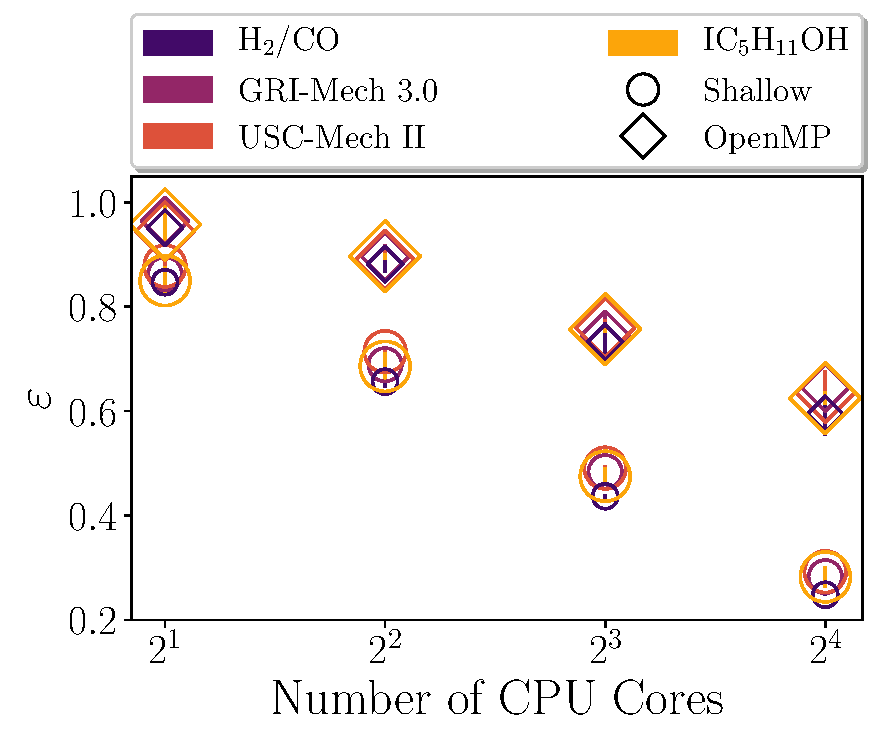
\includegraphics[width=\textwidth]{source_parallel_scaling.pdf}
      \caption{The strong parallel scaling efficiency (as defined in~\cref{e:strong_scaling}) of source-term evaluation for Intel OpenCL\slash OpenMP on the \avx/ machine.}
      \label{F:source_parallel_scaling}
  \end{subfigure}
  \hfill
  \begin{subfigure}[t]{0.48\linewidth}
      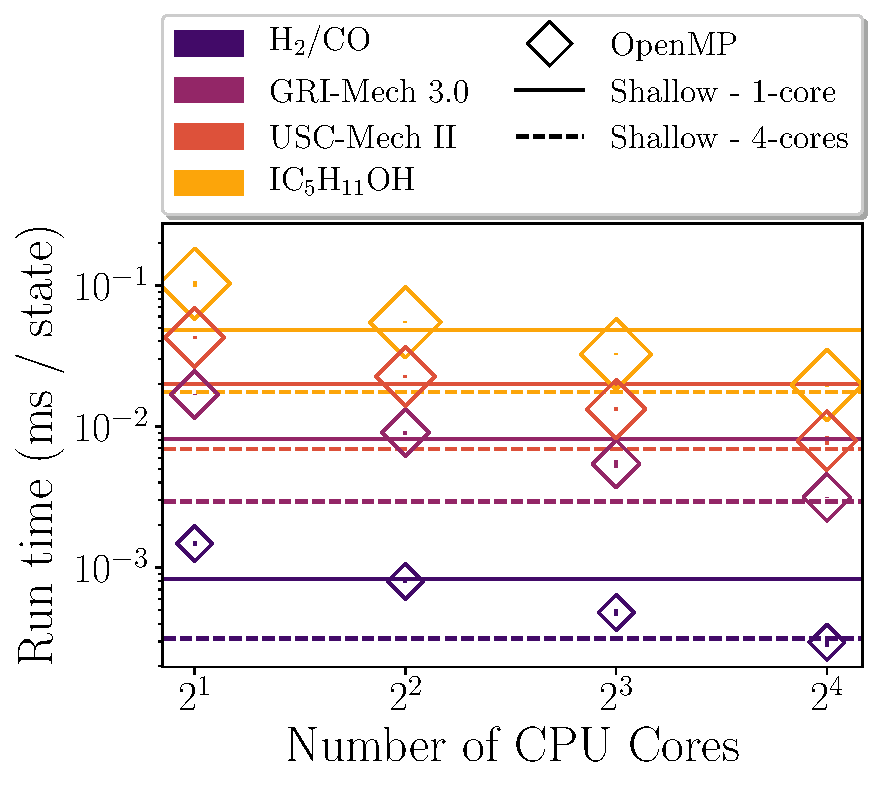
\includegraphics[width=\textwidth]{source_crossover.pdf}
      \caption{The mean run time per condition of OpenMP source-term evaluation on different cores compared to a shallow-vectorized Intel OpenCL evaluation on \num{1} (solid lines) and \num{4} (dashed lines) cores on \avx/ machine.}
      \label{F:source_crossover}
  \end{subfigure}
  \\
  \begin{subfigure}[t]{0.48\linewidth}
      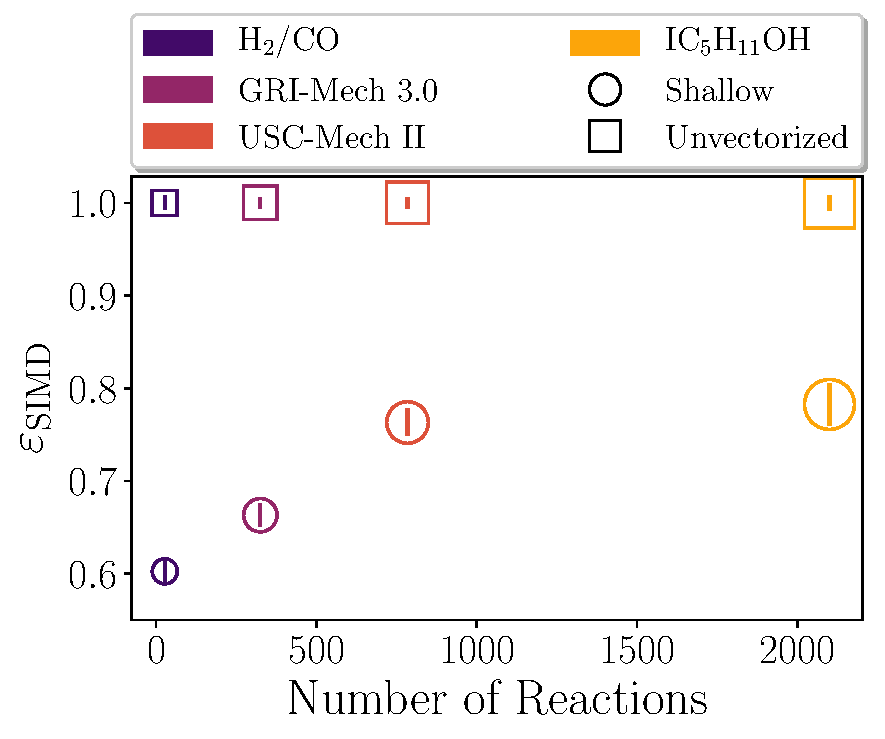
\includegraphics[width=\textwidth]{source_simd_efficiency.pdf}
      \caption{The SIMD efficiency (\cref{e:simd_efficiency}) of source-term evaluation for the Intel OpenCL runtime on a single core of the \avx/ CPU.}
      \label{F:source_simd_scaling}
  \end{subfigure}
  \hfill
  \begin{subfigure}[t]{0.48\linewidth}
      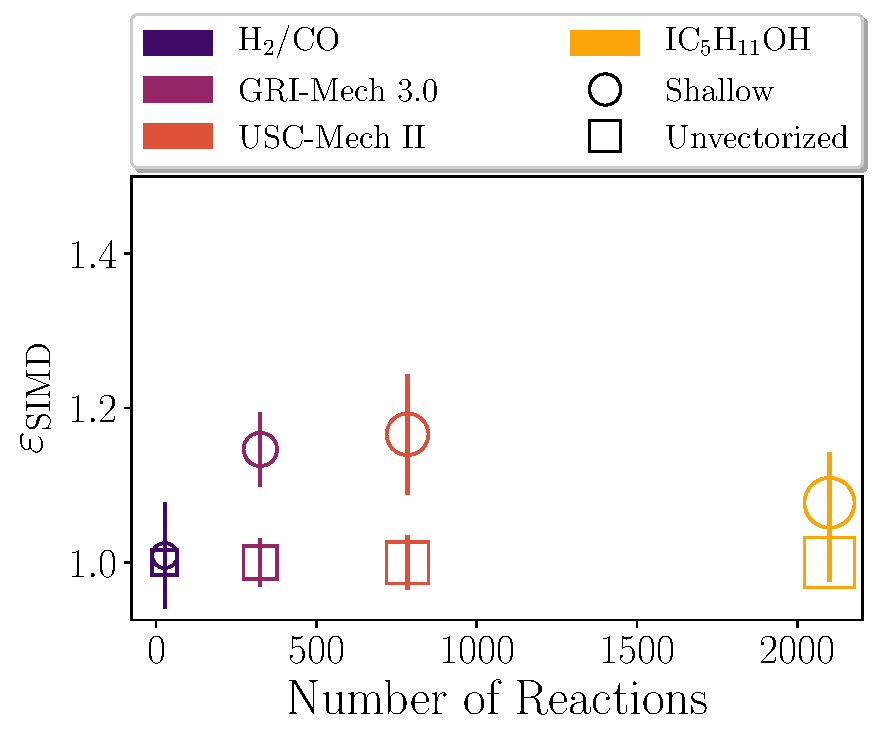
\includegraphics[width=\textwidth]{source_sse_simd_efficiency.pdf}
      \caption{The SIMD efficiency (\cref{e:simd_efficiency}) of source-term evaluation for the Intel OpenCL runtime on a single core of the \sse/ CPU.}
      \label{F:source_sse_simd_scaling}
  \end{subfigure}
  \caption{The parallel scaling efficiency and SIMD efficiency of source-term evaluation for Intel OpenCL on the \avx/ and \sse/ CPUs.}
  \label{F:source_scaling}
\end{figure}

\Cref{F:source_parallel_scaling} shows the strong parallel scaling efficiency of source-term evaluation in \texttt{pyJac} on the \avx/ machine for both the shallow-vectorized Intel OpenCL and OpenMP codes.
In general, the \ce{H2}\slash\ce{CO} mechanism has the worst scaling efficiency for both Intel OpenCL and OpenMP, likely resulting from both its relatively small size, and few falloff\slash chemically activated reaction (in particular, the additional expensive logarithm and exponential evaluations that accompany them); \add{as demonstrated in~\cref{S:SIMD_scaling} the amount of computational work required per thermochemical state plays a critical role in the full utilization of SIMD instructions\slash multiple threads}.
Additionally, OpenMP tends to have higher scalings than the shallow-vectorized OpenCL code, e.g., \textasciitilde\num{0.9} and \textasciitilde\num{0.75} for \num{4} and \num{8} CPU cores, respectively, compared to just \numrange{0.66}{0.72} and \numrange{0.44}{0.48} for OpenCL; although not pictured (to keep the figure readable), the unvectorized Intel OpenCL code has only slightly worse scaling than the OpenMP code, hence the poorer scaling is unique to the shallow-vectorizated code.
This is due in large part to the superior performance of the shallow-vectorized OpenCL code, coupled with the relatively small amounts of work associated with source-term evaluation.
To illustrate this,~\cref{F:source_crossover} shows the mean run time per-condition of the OpenMP source-term evaluations for \numrange{2}{16} cores, compared to the shallow-vectorized OpenCL code on \num{1} (solid line) and \num{4} (dashed line) cores on the \avx/ machine.
For all chemical models, the mean run time per-condition (and hence the computational work allocated per-core, one of the key-drivers of parallel scaling efficiency~\cite{strong_scaling}) of OpenMP running on \num{4} cores is roughly equal to that of the shallow-vectorized OpenCL code on a single core.
Similarly, OpenMP running on \num{16} cores is roughly equivalent to the OpenCL code on \num{4} cores.
Therefore, a more fair comparison of parallel scaling efficiencies is to compare OpenCL running on \num{4} cores, to OpenMP on \num{16}; the OpenMP code's parallel efficiency drops to \textasciitilde\num{0.64} for \num{16} cores, similar to OpenCL's parallel scaling efficiency of \numrange{0.66}{0.72} at \num{4} cores.
Indeed, as will be seen in~\cref{S:jacobian_results} the strong parallel scaling efficiency for sparse Jacobian evaluation---the most computationally intensive task in this work---are far more similar between Intel OpenCL and OpenMP.

The SIMD efficiency is defined as:
\begin{equation}
 \label{e:simd_efficiency}
 \varepsilon_{\text{SIMD}} = \frac{\bar{t}_{\text{unvec}}}{W \bar{t}_{\text{shallow}}}
\end{equation}
where $\bar{t}_{\text{unvec}}$ is the mean run time per condition of the unvectorized OpenCL code, $\bar{t}_{\text{shallow}}$ the same for the shallow-vectorized OpenCL code, and $W$, the vector-width reported in number of double operations in~\cref{t:cpus}.
This measure compares the actual speedup due to shallow-vectorization compared to the nominal vector-width of the machine in question.
\Cref{F:source_simd_scaling} shows the SIMD efficiency of source-term evaluation in \texttt{pyJac} on a single core of the \avx/ machine; the larger models (isopentanol and USC-Mech II) have higher SIMD efficiency of \numrange{0.76}{0.78}, and the smaller models (\ce{H2}\slash\ce{CO}, GRI-Mech \num{3.0}) have lower SIMD efficiency, \numrange{0.6}{0.66}.
This again demonstrates that the SIMD-vectorization becomes efficient as the amount of work to perform increases (with increasing model size).
Interestingly,~\cref{F:source_sse_simd_scaling} shows the SIMD efficiency on the \sse/ machine as greater than one; this is likely caused by a combination of use of an OpenCL vector-width greater than the native CPU vector-width (i.e., \num{8} versus \num{2}), and the improved data-locality for the vectorized-data ordering, as discussed in~\cref{S:data}, and results in a modest \SIrange{7}{17}{\percent} improvement over the nominal vector-width.


\subsubsection{Jacobian evaluation}
\label{S:jacobian_results}

\begin{figure}[htbp]
   \centering
  \begin{subfigure}[t]{0.48\linewidth}
      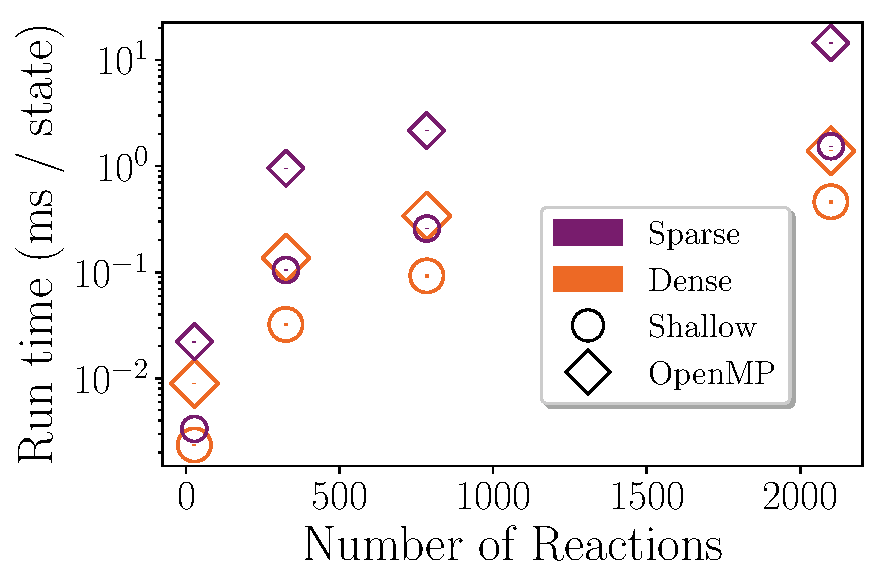
\includegraphics[width=\textwidth]{sparse_vs_dense.pdf}
      \caption{The mean run time per condition of sparse and dense Jacobian evaluations for Intel OpenCL\slash OpenMP on the \avx/ machine.}
      \label{F:sparse_vs_dense}
  \end{subfigure}
  \hfill
  \begin{subfigure}[t]{0.48\linewidth}
      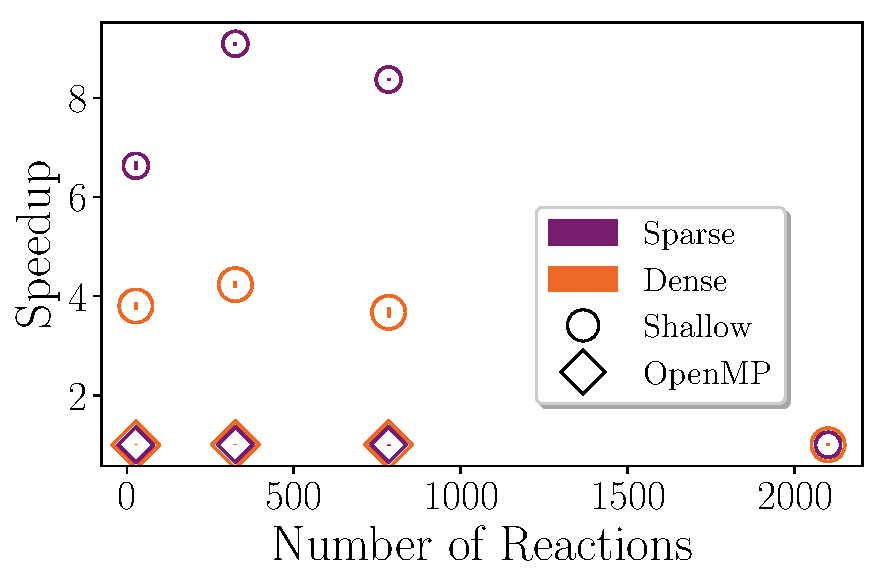
\includegraphics[width=\textwidth]{sparse_vs_dense_speedup.pdf}
      \caption{The speedup of the sparse and dense Jacobian evaluations for Intel OpenCL over the sparse\slash dense OpenMP baseline on the \avx/ machine.}
      \label{F:sparse_vs_dense_speedup}
  \end{subfigure}
  \\
  \begin{subfigure}[t]{0.48\linewidth}
      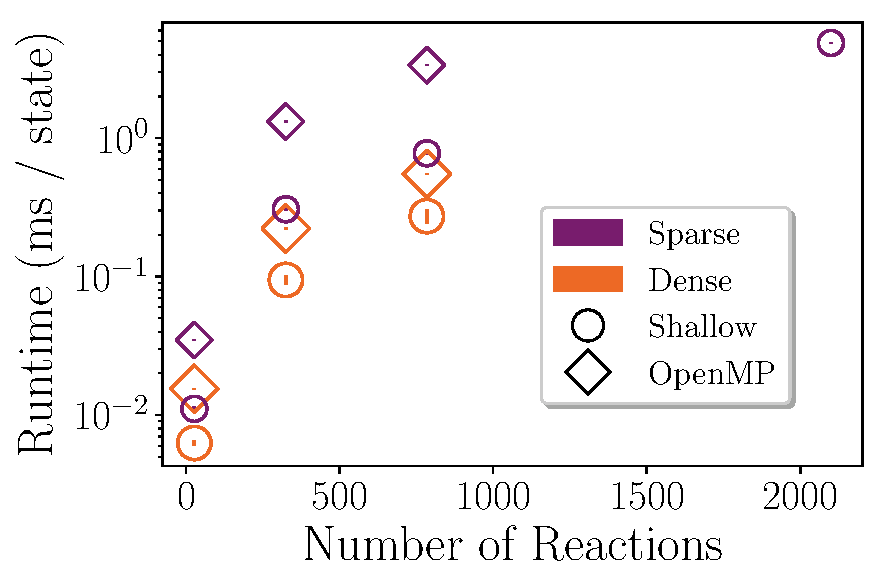
\includegraphics[width=\textwidth]{sparse_vs_dense_sse.pdf}
      \caption{The mean run time per condition of sparse and dense Jacobian evaluations for Intel OpenCL\slash OpenMP on the \sse/ machine.}
      \label{F:sparse_vs_dense_sse}
  \end{subfigure}
  \hfill
  \begin{subfigure}[t]{0.48\linewidth}
      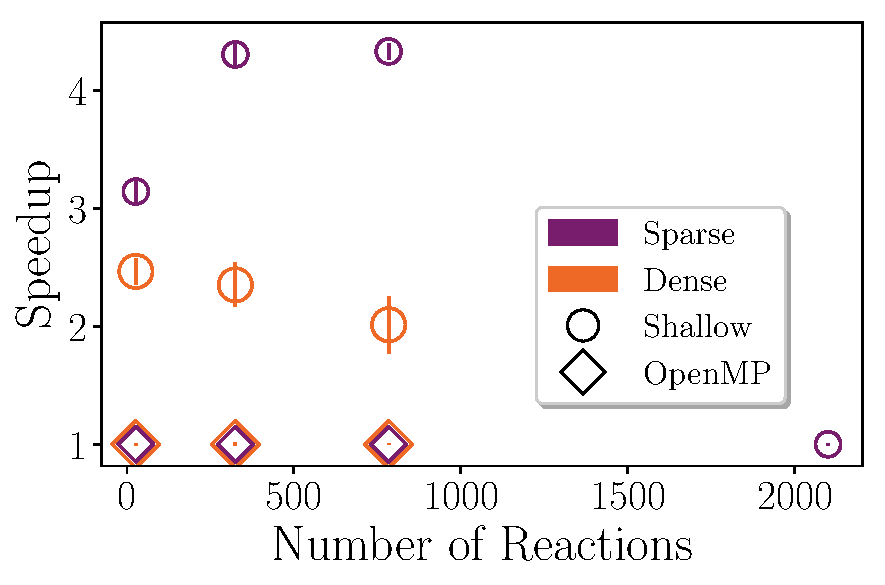
\includegraphics[width=\textwidth]{sparse_vs_dense_see_speedup.pdf}
      \caption{The speedup of the sparse and dense Jacobian evaluations for Intel OpenCL over the sparse\slash dense OpenMP baseline on the \sse/ machine.}
      \label{F:sparse_vs_dense_sse_speedup}
  \end{subfigure}
  \caption{Performance of sparse and dense Jacobian evaluations on the CPU platforms in \texttt{pyJac}.}
  \label{F:jacobian_perfomance}
\end{figure}

\Cref{F:jacobian_perfomance} shows the performance of the sparse and dense Jacobian evaluations in \texttt{pyJac} on the CPU platforms.
In~\cref{F:sparse_vs_dense}, the mean run time per condition is presented for the shallow-vectorized Intel OpenCL and OpenMP codes on the \avx/ CPU.
The sparse Jacobian evaluations are slower on both Intel OpenCL and OpenMP due to indirect lookup indexing requirements, as discussed in~\cref{S:sparsity}.
Interestingly the shallow-vectorized OpenCL code is less negatively impacted by the indirect lookup; the sparse OpenMP code is \SIrange{2.47}{10.42}{$\times$} slower than the dense OpenMP evaluation, while the sparse shallow-vectorized OpenCL code is just \SIrange{1.41}{3.34}{$\times$} slower than its dense counterpart.
As a result, the shallow-vectorized sparse OpenCL code is as fast, or faster than the dense OpenMP code in all cases on the \avx/ machine (\cref{F:sparse_vs_dense}).
\Cref{F:sparse_vs_dense_speedup} shows the speedup of the sparse\slash dense shallow-vectorized OpenCL over the same sparse\slash dense Jacobian format on OpenMP; the dense OpenCL code is \SIrange{3.03}{4.23}{$\times$} faster than the corresponding dense OpenMP code.
This speedup increases to \SIrange{6.63}{9.44}{$\times$} for the sparse Jacobian.

On the \sse/ machine,~\cref{F:sparse_vs_dense_sse} shows similar results; the sparse OpenMP code is the slowest in all cases, and the shallow-vectorized OpenCL code is nearly as fast as the dense OpenMP code.
Once again, the sparse OpenCL code is far less negatively impacted by the indirect lookup, and is only \SIrange{1.76}{3.33}{$\times$} slower than its dense counterpart, while the sparse OpenMP code is significantly (\SIrange{2.25}{8.72}{$\times$}) slower than the dense version.
In~\cref{F:sparse_vs_dense_sse_speedup}, the speedup of the sparse and dense shallow-vectorized OpenCL codes are compared to their OpenMP version; the dense OpenCL code is \SIrange{1.92}{2.47}{$\times$} faster, while the sparse shallow-vectorization achieves a speedup of \SIrange{3.14}{5.03}{$\times$}.

\begin{figure}[htbp]
   \centering
  \begin{subfigure}[t]{0.48\linewidth}
      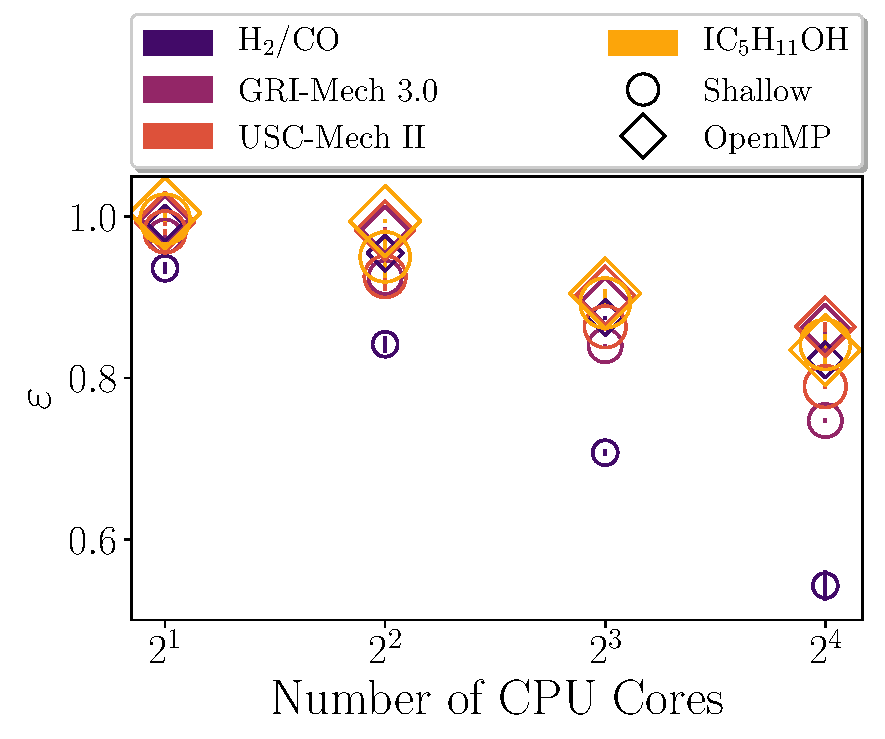
\includegraphics[width=\textwidth]{sparse_jac_scaling.pdf}
      \caption{Sparse Jacobian evaluation parallel scaling efficiency for Intel OpenCL\slash OpenMP on the \avx/ machine.}
      \label{F:sparse_jac_scaling}
  \end{subfigure}
  \hfill
  \begin{subfigure}[t]{0.48\linewidth}
      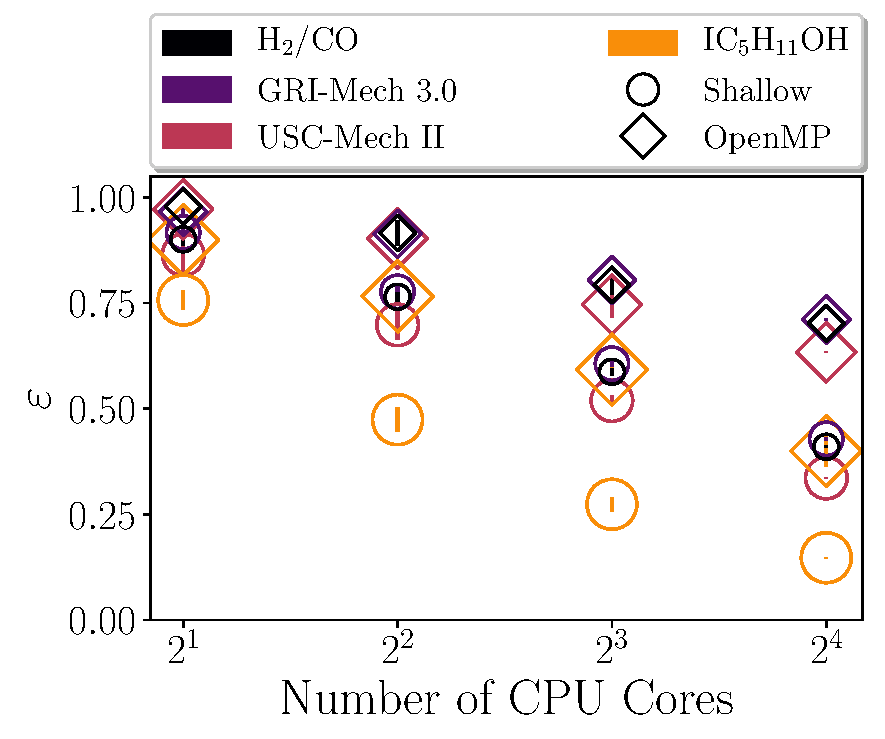
\includegraphics[width=\textwidth]{dense_jac_scaling.pdf}
      \caption{Dense Jacobian evaluation parallel scaling efficiency for Intel OpenCL\slash OpenMP on the \avx/ machine.}
      \label{F:dense_jac_scaling}
  \end{subfigure}
  \caption{The parallel scaling efficiencies of sparse and dense Jacobian evaluations for the shallow-vectorized Intel OpenCL and OpenMP codes on the \avx/ CPU.}
\end{figure}

In~\cref{F:sparse_jac_scaling}, the strong parallel scaling efficiency of the sparse shallow-vectorized OpenCL is compared to the sparse OpenMP code.
The plot is a bit difficult to read, as most of the data-points are clustered together, however the key takeaway is that the parallel scaling efficiency of the shallow-vectorized OpenCL code is very similar to that of the OpenMP code, in contrast to the parallel scaling efficiency of source-term evaluation (\cref{F:source_parallel_scaling}).
The \ce{H2}\slash\ce{CO} model has the worst scaling for both codes, ranging from \numrange{0.94}{0.54} and \numrange{0.99}{0.82} for OpenCL and OpenMP, respectively on \numrange{2}{16} cores.
As the model size increases, the efficiency of the OpenCL code improves dramatically, reaching \numrange{0.997}{0.84} for the isopentanol model.
\Cref{F:dense_jac_scaling} shows scaling for the shallow-vectorized dense Jacobian OpenCL code.
In this case, the isopentanol model has the worst scaling for both codes.
Tt is noted that due to the sheer size of the dense isopentanol Jacobian---storing the dense matrix for a single thermochemical state takes over \SI{1}{\mega\byte} of data---the total number of states for the dense isopentanol Jacobian evaluation was limited to \num{50000} (which requires over \SI{50}{\giga\byte} of memory); this greatly drops the computation cost for this case, and adversely affects the scaling efficiency as was discussed in~\cref{S:source_results}.
Excluding the isopentanol model, the dense shallow-vectorized OpenCL scalings are slightly higher than for source-term evaluation, e.g., \numrange{0.70}{0.78} and \numrange{0.52}{0.61} for \num{4} and \num{8} cores, respectively (compared to \numrange{0.66}{0.72} and \numrange{0.44}{0.48} for shallow-vectorized OpenCL source-term on the same \num{4} and \num{8} cores); this is due to the higher computational cost of Jacobian evaluation, and hence more available work per CPU-core.
As in~\cref{S:source_results}, we note that the shallow-vectorized dense Jacobian code running on \num{1} and \num{4} cores of the \avx/ machine is roughly as fast as the OpenMP code on \num{4} and \num{16} cores, respectively; the parallel scaling efficiency of OpenMP at \num{16} cores (excluding isopentanol as previously) is \numrange{0.63}{0.71}, similar to the shallow-vectorization's efficiency of \numrange{0.70}{0.78} for \num{4} cores.

\begin{figure}[htbp]
   \centering
  \begin{subfigure}[t]{0.48\linewidth}
      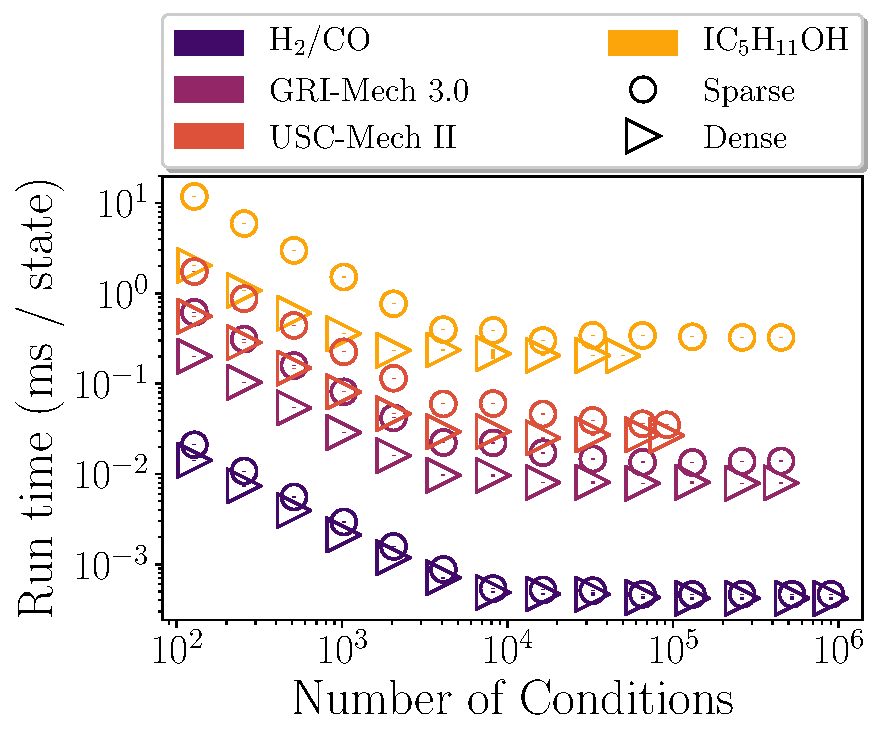
\includegraphics[width=\textwidth]{gpu_sparse_vs_dense.pdf}
      \caption{Mean run time per condition of sparse and dense Jacobian evaluations on the \gpunew/ GPU.}
      \label{F:gpu_sparse_vs_dense}
  \end{subfigure}
  \hfill
  \begin{subfigure}[t]{0.48\linewidth}
      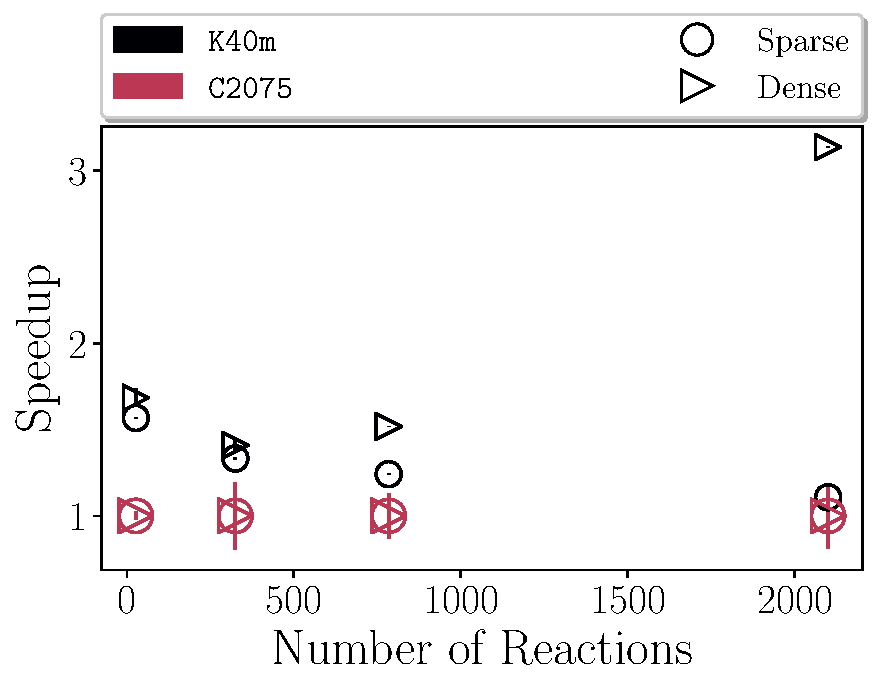
\includegraphics[width=\textwidth]{gpu_jacobian_speedup.pdf}
      \caption{Speedup of the \gpunew/ over \gpuold/ GPUs for sparse and dense Jacobian evaluations, normalized per-Jacobian type (i.e., sparse versus dense).}
      \label{F:gpu_jacobian_speedup}
  \end{subfigure}
  \caption{The performance of sparse\slash dense Jacobian evaluation on the \gpunew/ and \gpuold/ GPUs.}
\end{figure}

The mean run time per condition for the sparse and dense Jacobian evaluations on the \gpunew/ GPU is plotted in~\cref{F:gpu_sparse_vs_dense}.
As in the species evaluation case, the mean run time per condition drops steadily, for both cases becoming roughly constant after just \num{3e3} states (except for \ce{H2}\slash\ce{CO}, which levels off near \num{e4} conditions).
Sparse Jacobian evaluation is significantly slower for all models before the GPU becomes saturated (due to the indirect indexing lookup), however past the saturation point the performance gap between the sparse and dense evaluations narrows.
This is likely due to the ability to fit many more sparse Jacobian matrices in the \gpunew/'s memory, as well as improved data-locality\slash caching due to the smaller size of the sparse Jacobian.
\Cref{F:gpu_jacobian_speedup} presents the speedup of the \gpunew/ over the \gpuold/ GPU for sparse\slash dense Jacobian evaluation; sparse evaluation on the \gpunew/ is \SIrange{1.10}{1.59}{$\times$} faster than on the \gpuold/, while dense evaluation is \SIrange{1.36}{3.0}{$\times$} faster.
The speedup on the \gpunew/ appears to decrease with increasing mechanism size for the sparse evaluation, but increases for the larger models in dense evaluation; this is likely due to the larger available memory of the \gpunew/, and hence fewer data-transfer operations to\slash from the GPU.


In~\cref{F:fd_vs_analytical}, the performance of the sparse analytical-Jacobian is compared to a sparse first-order finite-difference Jacobian on both the \avx/ CPU and the \gpuold/ \gpunew/ GPUs.
\Cref{F:fd_vs_analytical_cpu} shows large speedups for both the OpenMP code and shallow-vectorized OpenCL code; the analytical OpenMP Jacobian is \SIrange{3.92}{8.67}{$\times$} faster, while the analytical OpenCL Jacobian achieves speedups of \SIrange{17.22}{55.11}{$\times$}.
It is noted that the isopentanol case was excluded here, as a single run of the sparse finite-difference Jacobian using either OpenCL or OpenMP took over \num{12} hours of run time.
In addition the current finite-difference formulation breaks Intel's auto-vectorizer, hence the OpenCL speedup comparison is made against the unvectorized OpenCL code; it is not a high priority to fix this issue, as the finite-difference Jacobian was implemented for comparison purposes only.
Although we do not display the dense finite-difference Jacobian speedup in~\cref{F:fd_vs_analytical_cpu}, the dense OpenCL and OpenMP analytical Jacobian codes out-perform the finite-difference variants by even larger margins; \SIrange{24.44}{245.63}{$\times$} for OpenCL, and \SIrange{9.68}{112.73}{$\times$} for OpenMP (these data do include the isopentanol model, though limited to \num{50000} conditions as discussed previously).
A comparison of the sparse analytical and finite-difference Jacobians on the GPUs is presented in~\cref{F:fd_vs_analytical_gpu}.
The analytical Jacobian on the \gpunew/ and \gpuold/ shows large speedups, increasing with chemical model size, in the range of \SIrange{3.81}{17.60}{$\times$}; the \gpunew/ has a larger speedup than the \gpuold/ (\SI{17.60}{$\times$} v.s., \SI{14.75}{$\times$}) for the isopentanol model due to its larger available memory.
Although not pictured, the dense analytical-Jacobian on the \gpunew/ GPU has larger speedups compared with the dense finite-difference Jacobian: \SIrange{4.04}{45.13}{$\times$}; the \gpunew/ GPU again has a significantly larger speedup than the \gpuold/ for the isopentanol model (\SI{45.13}{$\times$} versus \SI{23.85}{$\times$}), further underscoring the effect of the larger available memory on the \gpunew/.

\begin{figure}[htbp]
   \centering
  \begin{subfigure}[t]{0.48\linewidth}
      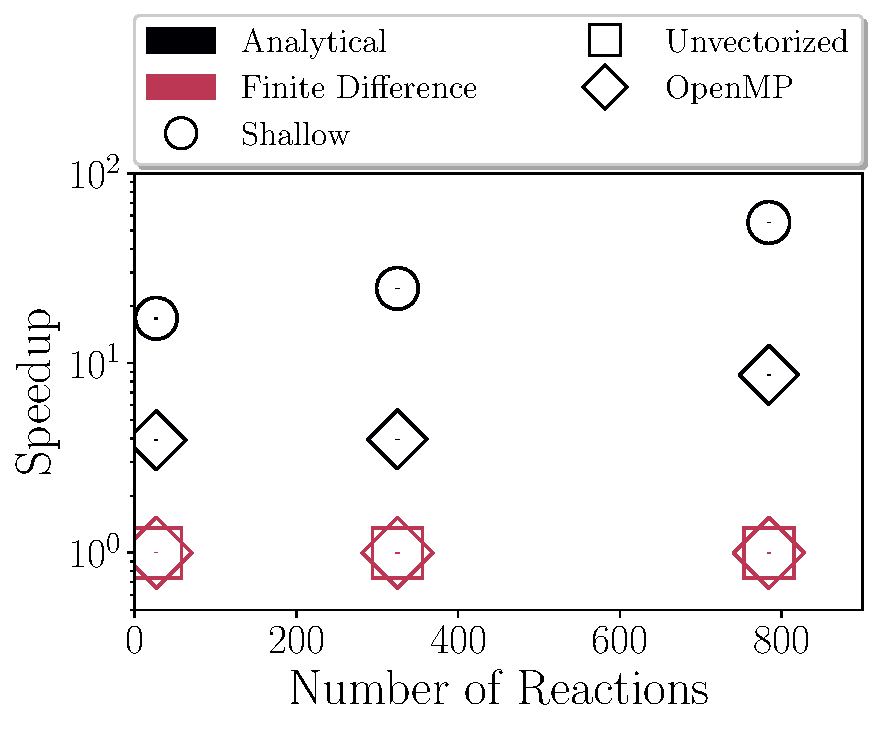
\includegraphics[width=\textwidth]{finite_difference_vs_analytical.pdf}
      \caption{Speedup of the sparse analytical Jacobian versus finite-difference Jacobian evaluation on the \avx/ CPU, normalized per-language}
      \label{F:fd_vs_analytical_cpu}
  \end{subfigure}
  \hfill
  \begin{subfigure}[t]{0.48\linewidth}
      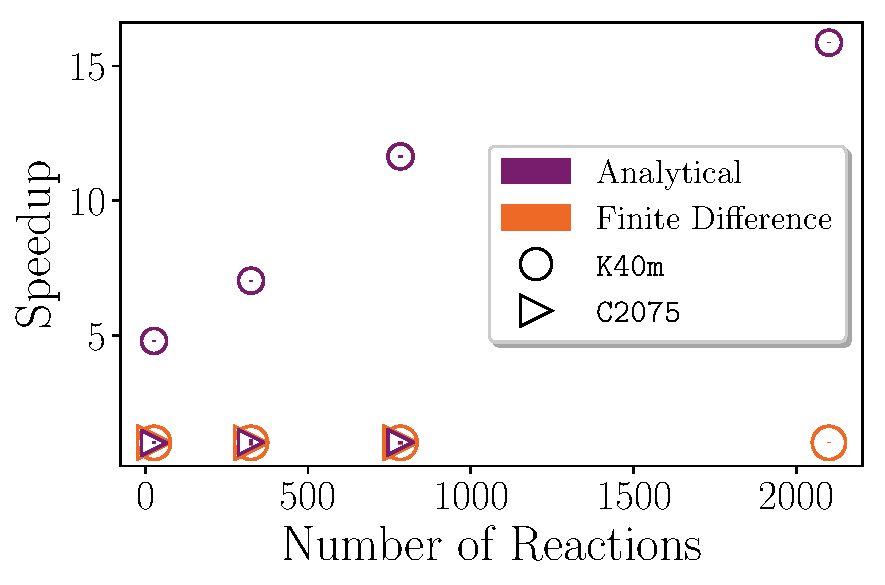
\includegraphics[width=\textwidth]{finite_difference_vs_analytical_gpu.pdf}
      \caption{Speedup of the analytical versus finite-difference Jacobian evaluation on both the \gpunew/ and \gpuold/ GPUs, normalized per-GPU}
      \label{F:fd_vs_analytical_gpu}
  \end{subfigure}
  \caption{The performance of a sparse, first-order forward finite-difference Jacobian compared to the analytical Jacobian on the \avx/ CPU and both GPUs.}
  \label{F:fd_vs_analytical}
\end{figure}

\Cref{F:v1_vs_v2} compares the performance for evaluation of the dense-analytical Jacobian of the new version of \texttt{pyJac}, \texttt{pyJac-v2}, to the previous version, \texttt{pyJac-v1} \cite{pyjac16}, on the \sse/ CPU and \gpuold/ GPU; dense Jacobian evaluation was selected as it was the only type implemented in the previous version of \texttt{pyJac}.
On the \sse/ CPU, the \texttt{pyJac-v2} is faster than \texttt{pyJac-v1} for OpenMP evaluation for the larger chemical models; the static OpenMP code generated by \texttt{pyJac-v1} (see~\cref{s:unittest}) is \SI{1.79}{$\times$} faster for the \ce{H2}\slash\ce{CO} model, and only \SI{1.09}{$\times$} slower for the GRI-Mech 3.0 model.
In contrast, the loop-based OpenMP code of \texttt{pyJac-v2} is \SIrange{3.37}{10.19}{$\times$} faster than \texttt{pyJac-v1} for the USC-Mech II and isopentanol models.
The shallow-vectorized OpenCL code is faster than \texttt{pyJac-v1} in all cases, achieving speedups of \SIrange{1.37}{19.56}{$\times$} increasing with model size.
In~\cref{F:v1_vs_v2_gpu}, the performance of the \texttt{pyJac-v2} dense-analytical Jacobian on the \gpuold/ GPU is compared to \texttt{pyJac-v1} on the same.
As with the CPU, the static code of \texttt{pyJac-v1} is slightly faster for the \ce{H2}\slash\ce{CO} model, however \texttt{pyJac-v2} outperforms \texttt{pyJac-v1} by \SIrange{1.25}{2.84}{$\times$} for the other models; it is noted that the decrease in speedup for the isopentanol model is likely due to the limited number of conditions in dense-evaluation for \texttt{pyJac-v2}, as noted earlier.

\begin{figure}[htbp]
   \centering
  \begin{subfigure}[t]{0.48\linewidth}
      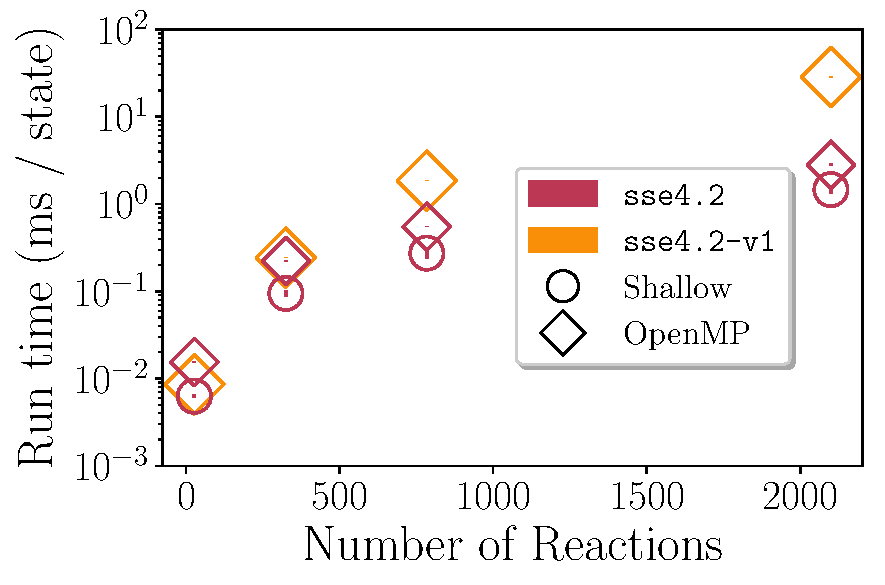
\includegraphics[width=\textwidth]{v1_vs_v2.pdf}
      \caption{Speedup of dense Jacobian evaluation in \texttt{pyJac-v2} over \texttt{pyJac-v1} on the \sse/ CPU}
      \label{F:v1_vs_v2_cpu}
  \end{subfigure}
  \hfill
  \begin{subfigure}[t]{0.48\linewidth}
      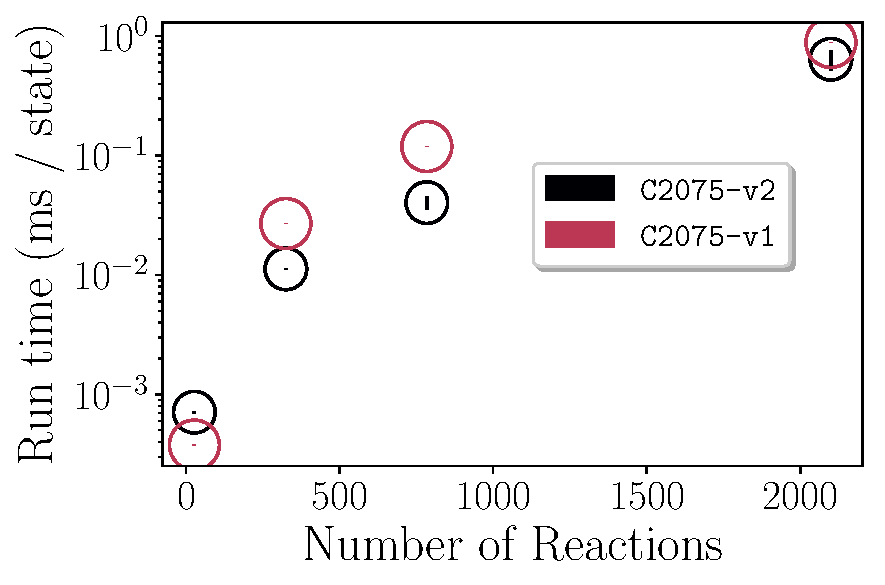
\includegraphics[width=\textwidth]{v1_vs_v2_gpu.pdf}
      \caption{Speedup of dense Jacobian evaluation in \texttt{pyJac-v2} over \texttt{pyJac-v1} on the \gpuold/ GPU}
      \label{F:v1_vs_v2_gpu}
  \end{subfigure}
  \caption{Performance comparison of the new version of \texttt{pyJac} (\texttt{v2}) and the previous version, \texttt{v1}~\cite{pyjac16}.}
  \label{F:v1_vs_v2}
\end{figure}

\section{Conclusions}
In this work, automatically generated OpenCL codes for SIMD\slash SIMT-vectorized thermochemical source-term and sparse\slash dense chemical kinetic Jacobian evaluation were developed and validated for a range of chemical kinetic models~\cite{Burke:2011fh,smith_gri-mech_30,Wang:2007,Sarathy:2013jr} and multiple CPUs\slash GPUs (\cref{t:cpus,t:gpus}).
\add{Reviewing the goals of this work, as discussed in~\cref{S:Goals}}:

\subsection{Derive and validate a new Jacobian formulation for \texttt{pyJac} that greatly increases sparsity}
A new formulation resulted in highly sparse (\SIrange{28.6}{88.5}{\percent}) chemical kinetic Jacobians, with options to futher increase sparsity (to \SIrange{31.66}{92.0}{\percent}) at the expense of strict correctness.

\subsection{Enable cross-platform SIMD\slash SIMT vectorization for the CPU, GPU and other accelerators}
\add{Shallow-vectorized evaluation of \texttt{pyJac}'s chemical kinetic source-term and analytical Jacobian was demonstrated on both the CPU and GPU via OpenCL.}
Deep-vectorization, though possible on the Portable OpenCL (POCL) platform~\cite{poclIJPP}, did not yield any performance benefit as POCL did not achieve vectorizations for any execution pattern studied; deep-vectorization deserves further study with other platforms (e.g., CUDA).
\add{In addition, parallel OpenMP evaluation was demonstrated on the CPU.}

\subsection{Investigate the performance for a wide range chemical kinetic models, specifically looking at speedups due to SIMD\slash SIMT-vectorization as well as relative to the previous version of \texttt{pyJac}}

Significant speedups in shallow SIMD-vectorized source-term evaluation over a parallel OpenMP code were demonstrated, up to \SIrange{2.53}{2.92}{$\times$} and \SIrange{3.40}{4.08}{$\times$} for \sse/ and \avx/ capable CPUs; in addition, source-term evaluation was \SIrange{1.40}{1.88}{$\times$} faster on a \gpunew/ GPU compared to a \gpuold/ GPU.
Vectorized data-orderings specifically formulated for shallow\slash deep SIMD\slash SIMT vectorizations were proposed, resulting in a shallow-vectorized speedup of \SIrange{2.14}{2.58}{$\times$} over a more standard ``F''-ordered (column major) shallow-vectorization; when compared to the corresponding speedup of \SIrange{1.35}{2.09}{$\times$} for the ``C''-ordered (row major) OpenMP code over an ``F''-ordered equivalent, the value of the vectorized data-ordering is evident.
In addition, the choice of \conp/\slash\conv/ formulation was determined to be negligible on source-term evaluations, while varying the OpenCL vector-width had only modest (\textasciitilde\SI{10}{$\percent$}) performance effects on both the CPU and GPU.
The strong parallel scaling efficiency was also examined for source-term evaluation; the parallel OpenMP code generally had better efficiencies, but when compared to a shallow-vectorized code with roughly equivalent performance---e.g., source-term shallow-vectorized evaluation on \num{4} cores to \num{16} OpenMP cores---the scalings were similar.
Examination of SIMD efficiency revealed increasing speedups with chemical model-size for source-term evaluation on the \avx/ CPU, while on the \sse/ CPU speedups larger than the nominal vector-width were achieved.

The performance of sparse and dense Jacobian evaluation was also characterized on the CPU\slash GPU platforms.
The sparse shallow-vectorized OpenCL code was \SIrange{6.63}{9.44}{$\times$} and \SIrange{3.14}{5.03}{$\times$} faster than OpenMP evaluation on the \avx/ and \sse/ CPUs, respectively, while dense shallow-vectorized evaluation was \SIrange{3.03}{4.23}{$\times$} and \SIrange{1.92}{2.47}{$\times$} faster on the same.
Sparse Jacobian evaluation was slower than dense evaluation on all CPU\slash GPU platforms due to indirect lookup requirements in array indexing, however the shallow-vectorized OpenCL code was less adversely affected---a slowdown of \SIrange{1.41}{3.34}{$\times$} on the \avx/ CPU---than OpenMP, which was \SIrange{2.47}{10.42}{$\times$} slower on the same.
On the \gpunew/ GPU, sparse evaluation was \SIrange{1.10}{1.59}{$\times$} faster than on the \gpuold/ GPU, while dense evaluation was \SIrange{1.36}{3.0}{$\times$} faster; the use of OpenCL Image\slash CUDA Texture memory to accelerate the indirect lookup for sparse matrix evaluation should be investigated in the future.
Analytical Jacobian evaluation was significantly faster than a first-order finite-difference based approach on all platforms, achieving speedups of \SIrange{3.81}{17.60}{$\times$} and \SIrange{4.04}{45.13}{$\times$} for sparse and dense evaluation (respectively) on the GPUs; on the \avx/ CPU analytical evaluation was \SIrange{3.92}{55.11}{$\times$} and \SIrange{9.68}{245.63}{$\times$} for sparse and dense Jacobian evaluation (respectively) with OpenMP\slash shallow-vectorized OpenCL.
Finally, the performance of dense analytical-Jacobian evaluation in this new version of \texttt{pyJac} was compared to the previous version~\cite{pyjac16} on the \sse/\slash\gpuold/ CPU\slash GPU; OpenMP evaluation on the \sse/ CPU was \SI{1.79}{$\times$} slower for the smallest chemical model, but \SIrange{3.37}{10.19}{$\times$} faster for the larger models, while the shallow-vectorized OpenCL code was \SIrange{1.37}{19.56}{$\times$} faster than the previous version over all chemical models.
Similarly, evaluation on the \gpuold/ GPU was \SI{1.89}{$\times$} slower for the smallest model but \SIrange{1.25}{2.84}{$\times$} faster for the larger models.

\subsection{Future extensions to this work and practical notes on OpenCL usage}
\label{S:future}

It is important to note that while OpenCL provides an simple interface to enable cross-platform execution, and significant speedups were achieved via shallow-vectorized OpenCL code in this work, there are some serious potential pit-falls in its use.
The closed source OpenCL runtimes tested in this work (Intel and Nvidia) contain several bugs that result in compilation failures, simply incorrect vectorized machine code or even segmentation faults.
Further, these runtimes (in our experience) tend to be less responsive to fixing said bugs, with relatively infrequent new releases (or in Nvidia's case, lack of changelogs\slash public records of bug-fixes).
On the other hand, the open-source OpenCL runtime used in this work, POCL, has (in our experience) far fewer implementation bugs, and when issues arise the community is very responsive to bug reports and user outreach; however, POCL fails to achieve vectorization as noted in~\cref{S:source_results}.

As demonstration of the type of issue discussed, a minimum working example has been created~\cite{Nvidia_mwe} that demonstrates a failure of Nvidia's OpenCL runtime corresponding to the GPU driver version \num{375.26} on a Tesla \gpunew/ GPU; by simply changing to another runtime (e.g., Intel)---with no code changes or recompilation---the correct result can be found.
This provides a particularly vexing problem for the programmer, as there is often little that can be done to resolve the issue; thankfully, in this case we were able to upgrade the driver version to resolve the problem.
Further, as noted throughout this work certain code-generation patterns can break OpenCL execution\slash vectorization, e.g., the failure of POCL to achieve vectorization or Intel OpenCL's failure to vectorize the finite-difference Jacobian.
Indeed the vectorization process attempted by most OpenCL runtimes (and thus, reasons for incorrect\slash unvectorized code-output) is obscured from the user, making reasoning about errors or performance trends quite difficult.

Thankfully, \texttt{loo.py} allows relatively easy switching between output languages; the most significant code change requires building of the wrapper that initializes\slash transfers memory and calls the source-rate\slash Jacobian kernel.
Indeed, the OpenMP code-generation built into \texttt{pyJac} is currently only capable of parallel-execution, but extending this platform to shallow\slash deep-vectorizations (via \texttt{loo.py} and compiler \texttt{\#pragma}s) is a key priority going forwards as OpenMP is a standard library on most machines.
In addition, CUDA~\cite{Nvidia:2018} has been significantly more reliable in previous works~\cite{Niemeyer:2016aa,CurtisGPU:2017}, while Intel's open-source OpenCL alternative, ISPC~\cite{pharr2012ispc}, has been relatively stable and easy to work with during preliminary efforts with the unit-testing discussed in~\cref{s:unittest}.
The current deep-vectorization formulation would be executable for both CUDA and ISPC targets, as these languages implement double-precision atomic operations, further recommending their use.
It is also possible, particularly for the Intel OpenCL\slash POCL runtimes, that better performance\slash stability might be achieved using so-called ``explicit'' vectorization, i.e., through use of built-in vector types such as the \texttt{double8}; \add{specifically this change is hoped to enable vectorization on the POCL runtime} and might also enable deep-vectorization on the Intel OpenCL runtime.
\add{Finally, future extensions of this work will include additional target-languages (vectorized OpenMP, CUDA, ISPC, etc.) to improve ease of use and reliability, as well as improvements to the existing OpenCL targets, e.g., to enable meaningful deep-vectorized evaluation, as well the implementation of reaction sorting~\cite{Sewerin20151375} to improve SIMD-efficiency (\cref{S:SIMD_scaling}).}

One key-component missing in this current version of \texttt{pyJac} is vectorized sparse\slash dense linear-algebra subroutines to maximize the performance of LU-factorization and matrix-vector multiplication (commonly used in implicit-integration techniques).
Third-party\slash open-source options exist for some target-languages, e.g., cuBLAS~\cite{cublas}, clBLAS\slash clSPARSE~\cite{clmath} or SuperLU~\cite{superlu99}, but these do not necessarily cover all targets\slash required linear-algebra operations and, in the case of the CUDA\slash OpenCL libraries, are often optimized operation on one large matrix instead of many (relatively) smaller matrices.
The extent to which these existing programs may be used needs to be assessed and missing operations should be implemented in \texttt{loo.py} to ensure easy switching between target-languages\slash vectorization types.

\section{Acknowledgments}
This material is based upon work supported by the National Science Foundation
under grants ACI-1534688 (Curtis and Sung) and ACI-1535065 (Niemeyer).

\pagebreak

%% The Appendices part starts with the command \appendix;
%% appendix sections are then done as normal sections
\appendix
\setcounter{figure}{0}
\setcounter{table}{0}

% Fix for missing space between "Appendix" and letter
\renewcommand*{\thesection}{\appendixname~\Alph{section}}

\section{Jacobian error statistics per test-platform}
\label{A:per_platform}

This section gives more detail on the results presented in~\cref{S:jac_valid}, breaking down the reported error statistics per test-platform\slash language.
The error of the Intel OpenCL runtime is presented in~\cref{T:intel_error}, the Portable OpenCL (POCL) runtime in~\cref{T:pocl_error}, OpenMP in~\cref{T:omp_error} and the Nvidia OpenCL runtime in~\cref{T:nv_error}.
POCL and OpenMP tend to have the smallest error norms, while Nvidia tends to have the largest; in particular the stringent filtered error norm $E_{\mathcal{C} = 10^{20}}$ is two orders of magnitude larger for the Nvidia runtime than the other test platforms with the \ce{H2}\slash\ce{CO} and USC-Mech II models.

\begin{table}[htbp]
\sisetup{retain-zero-exponent=true}
\centering
\begin{tabular}{@{}l S[table-format=.0] S[table-format=1.3e1] S[table-format=1.3e1] S[table-format=1.3e1] S[table-format=1.3e1] @{}}
\toprule
Model                 & \multicolumn{1}{c}{$E_{\mathcal{L}}$} & \multicolumn{1}{c}{$E_{\mathcal{C} = 10^{20}}$}   & \multicolumn{1}{c}{$E_{\mathcal{C} = 10^{15}}$} \\
\midrule
\ce{H2}\slash \ce{CO} & \num{1.455e-14}      & \num{8.084e-01}  & \num{1.907e-05} \\
GRI-Mech 3.0          & \num{1.567e-14}      & \num{1.469e-07}  & \num{1.316e-07} \\
USC-Mech II           & \num{9.632e-15}      & \num{5.567e-03}  & \num{1.704e-07} \\
\ce{iC5H11OH}         & \num{1.227e-10}      & \num{1.363e-03}  & \num{2.864e-05} \\
\bottomrule
\end{tabular}
\caption{Summary of Jacobian matrix validation results for the Intel OpenCL runtime.
The reported error statistics are the maximum filtered relative error $E_\mathcal{C}$ and LAPACK error $E_{\mathcal{L}}$ over all vectorization patterns (\cref{t:platforms}),  \conp/\slash \conv/ and sparse\slash dense Jacobians.
The threshold for the filtered relative error is the same as reported in~\cref{S:jac_valid}.
}
\label{T:intel_error}
\end{table}

\begin{table}[htbp]
\sisetup{retain-zero-exponent=true}
\centering
\begin{tabular}{@{}l S[table-format=.0] S[table-format=1.3e1] S[table-format=1.3e1] S[table-format=1.3e1] S[table-format=1.3e1] @{}}
\toprule
Model                 & \multicolumn{1}{c}{$E_{\mathcal{L}}$} & \multicolumn{1}{c}{$E_{\mathcal{C} = 10^{20}}$}   & \multicolumn{1}{c}{$E_{\mathcal{C} = 10^{15}}$} \\
\midrule
\ce{H2}\slash \ce{CO} & \num{1.456e-14}      & \num{1.230e-01}  & \num{3.951e-06} \\
GRI-Mech 3.0          & \num{1.014e-14}      & \num{1.890e-07}  & \num{1.877e-07} \\
USC-Mech II           & \num{9.632e-15}      & \num{8.998e-04}  & \num{1.201e-08} \\
\ce{iC5H11OH}         & \num{9.133e-15}      & \num{1.723e-05}  & \num{5.108e-07} \\
\bottomrule
\end{tabular}
\caption{Summary of Jacobian matrix validation results for the Portable OpenCL (POCL) runtime.
The reported error statistics are the maximum filtered relative error $E_\mathcal{C}$ and LAPACK error $E_{\mathcal{L}}$ over all vectorization patterns (\cref{t:platforms}),  \conp/\slash \conv/ and sparse\slash dense Jacobians.
The threshold for the filtered relative error is the same as reported in~\cref{S:jac_valid}.
}
\label{T:pocl_error}
\end{table}

\begin{table}[htbp]
\sisetup{retain-zero-exponent=true}
\centering
\begin{tabular}{@{}l S[table-format=.0] S[table-format=1.3e1] S[table-format=1.3e1] S[table-format=1.3e1] S[table-format=1.3e1] @{}}
\toprule
Model                 & \multicolumn{1}{c}{$E_{\mathcal{L}}$} & \multicolumn{1}{c}{$E_{\mathcal{C} = 10^{20}}$}   & \multicolumn{1}{c}{$E_{\mathcal{C} = 10^{15}}$} \\
\midrule
\ce{H2}\slash \ce{CO} & \num{5.962e-15}      & \num{3.614e-02}  & \num{1.657e-06} \\
GRI-Mech 3.0          & \num{1.297e-15}      & \num{1.321e-07}  & \num{1.316e-07} \\
USC-Mech II           & \num{9.630e-15}      & \num{4.185e-04}  & \num{6.746e-09} \\
\ce{iC5H11OH}         & \num{6.131e-15}      & \num{1.721e-05}  & \num{5.108e-07} \\
\bottomrule
\end{tabular}
\caption{Summary of Jacobian matrix validation results for OpenMP execution.
The reported error statistics are the maximum filtered relative error $E_\mathcal{C}$ and LAPACK error $E_{\mathcal{L}}$ over all vectorization patterns (\cref{t:platforms}),  \conp/\slash \conv/ and sparse\slash dense Jacobians.
The threshold for the filtered relative error is the same as reported in~\cref{S:jac_valid}.
}
\label{T:omp_error}
\end{table}

\begin{table}[htbp]
\sisetup{retain-zero-exponent=true}
\centering
\begin{tabular}{@{}l S[table-format=.0] S[table-format=1.3e1] S[table-format=1.3e1] S[table-format=1.3e1] S[table-format=1.3e1] @{}}
\toprule
Model                 & \multicolumn{1}{c}{$E_{\mathcal{L}}$} & \multicolumn{1}{c}{$E_{\mathcal{C} = 10^{20}}$}   & \multicolumn{1}{c}{$E_{\mathcal{C} = 10^{15}}$} \\
\midrule
\ce{H2}\slash \ce{CO} & \num{1.862e-14}      & \num{1.741e+00}  & \num{4.508e-05} \\
GRI-Mech 3.0          & \num{1.489e-14}      & \num{3.842e-07}  & \num{3.687e-07} \\
USC-Mech II           & \num{1.174e-14}      & \num{1.119e-02}  & \num{1.983e-07} \\
\ce{iC5H11OH}         & \num{8.602e-15}      & \num{1.748e-05}  & \num{5.109e-07} \\
\bottomrule
\end{tabular}
\caption{Summary of Jacobian matrix validation results for Nvidia OpenCL execution.
The reported error statistics are the maximum filtered relative error $E_\mathcal{C}$ and LAPACK error $E_{\mathcal{L}}$ over all vectorization patterns (\cref{t:platforms}),  \conp/\slash \conv/ and sparse\slash dense Jacobians.
The threshold for the filtered relative error is the same as reported in~\cref{S:jac_valid}.
}
\label{T:nv_error}
\end{table}

\section{SIMD efficiency Scaling Example}
\label{S:SIMD_scaling}
\add{This simple example demonstrates the dependency of the SIMD efficiency of shallow-vectorized OpenCL source-term evaluation on the size of the chemical model in question, i.e., the amount of computational work per source-term evaluation.}
\add{The base chemical model for this example was the isopentanol model~\cite{Sarathy:2013jr} used throughout this work, and the same thermochemical state database described in~\cref{s:test_platforms} was used for source-term evaluation.}
\add{As in~\cref{S:results} all reported results are based on \num{10} individual runs and in this example all cases were run on the \avx/ machine using the Intel OpenCL runtime.}

\begin{algorithm}[htbp]
\algnewcommand\algorithmicinput{\textbf{Input:}}
\algnewcommand\INPUT{\item[\algorithmicinput]}
\begin{algorithmic}[0]
  \caption{A greedy selection algorithm to remove reactions from a base chemical model $M$, while preserving the number of active species.}
  \label{a:model_gen}
  \INPUT{Base chemical model $M$ with reactions $R$ and species $S$}
  \Function{Determine Species Count}{\text{active}}
    \For {Species $S_k$ in model $M$}
      \State  $\text{species\smallunderscore{}rxn\smallunderscore{}count}\left[k\right] \gets 0$
      \For {Reaction $R_j$ in model $M$}
	\If{$\text{active}[j]$ and $\left(\left\lvert \nu_{k, j}^{\prime}\right\rvert + \left\lvert \nu_{k, j}^{\prime\prime} \right\rvert \right) > 0$}
	  \State $\text{species\smallunderscore{}rxn\smallunderscore{}count}[k] \gets \text{species\smallunderscore{}rxn\smallunderscore{}count}[k] + 1$
	\EndIf
      \EndFor
    \EndFor
    \Return \text{species\smallunderscore{}rxn\smallunderscore{}count}
  \EndFunction
  \Procedure{Model Generation}{$M$}
  \State $\text{active}[j] \gets \text{True}$ for all reactions $R_j$ in $M$
  \State $\text{species\smallunderscore{}rxn\smallunderscore{}count}\gets \Call{Determine Species Count}{\text{active}}$
  \While {$\operatorname{min}\left(\text{species\smallunderscore rxn\smallunderscore count}\right) \ge 1$}
     \State $\text{species\smallunderscore{}rxn\smallunderscore{}count}\gets \Call{Determine Species Count}{\text{active}}$
     \For {Reaction $R_j$ in model $M$}
	\State $\text{rxn\smallunderscore{}count}[j] \gets \min_{\forall S_k \in R_j}{\left(\text{species\smallunderscore{}rxn\smallunderscore{}count}\left[k\right]\right)}$
     \EndFor
     \State $\text{remove\smallunderscore{}at} \gets \operatorname{argmax}\left(\text{rxn\smallunderscore{}count}\right)$
     \State $\text{active}[\text{remove\smallunderscore{}at}] \gets \text{False}$
  \EndWhile
  \EndProcedure
\end{algorithmic}
\end{algorithm}

\add{First, the reactions in the isopentanol model were converted to simple reversible Arrhenius reactions by either simply dropping third-body efficiency calculations (third-body enhanced reactions), using the high pressure-limit coefficients (falloff\slash chemically-activated and P-Log reactions) or fitting Arrenhius parameters to the calculated rate constant at a fixed pressure (chebyshev reactions).}
\add{This conversion made the cost of reaction rate evaluation roughly equivalent between all reactions in model, separating the effect of chemical model size from computational intensities of different reaction types on the SIMD efficiency.}
\add{Next, a greedy reaction removal algorithm (\cref{a:model_gen}) was utilized to generate a number of models ranging from \numrange{2100}{186} reactions, in increments of 200 reactions (except the final increment from \num{200} to \num{186} reactions).}

\begin{figure}[htbp]
\centering
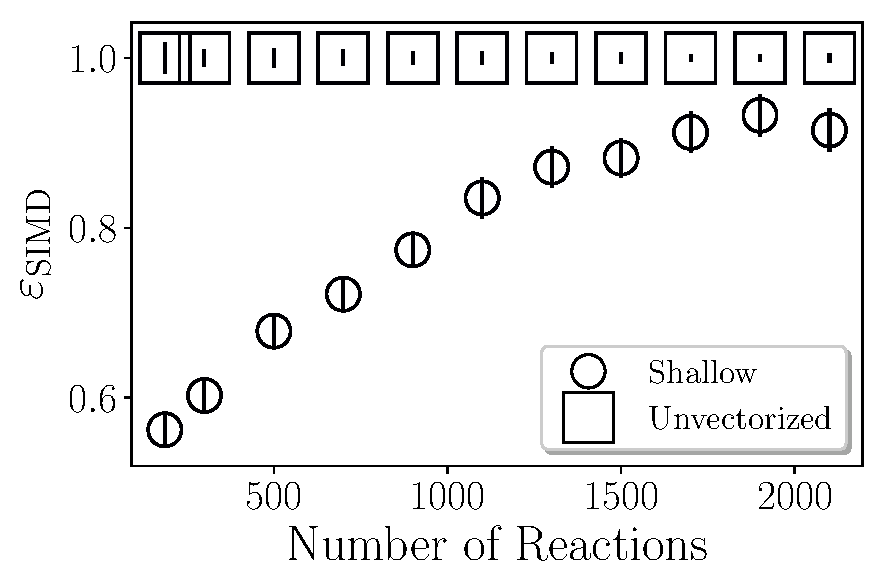
\includegraphics[width=0.5\linewidth]{simd_efficiency_scaling}
\caption{The effect on SIMD efficiency of varying chemical model size}
\label{F:simd_vs_rxns}
\end{figure}

\add{In order to discern the effect of varying chemical model size on the SIMD efficiency, shallow-vectorized and unvectorized source-term evaluation performance tests were run.}
\add{As demonstrated in~\cref{F:simd_vs_rxns} the SIMD efficiency is strongly dependent on the generated model size and and thus, amount of computational work per thermochemical state.}
\add{In addition, the range of SIMD efficiency in this example (\numrange{0.56}{0.91}) is larger than the range of SIMD efficiencies calculated for real chemical models, as seen in~\cref{F:source_simd_scaling}.}
\add{For smaller models---e.g., \ce{H2}\slash\ce{CO} which had a SIMD efficiency of \num{0.6} on the \avx/ CPU---this suggests that the presence of more computationally intensive fall-off\slash chemically activated reactions in model can increase the SIMD efficiency.}
\add{However, the base isopentanol model achieved a SIMD efficiency of only \num{0.78} on the \avx/ machine in~\cref{S:source_results}, suggesting that more work could be done to optimize the source-term evaluations.}
\add{In particular, it's likely that a reaction sorting method, such as suggested by Sewerin and Rigopoulos~\cite{Sewerin20151375}, would be particularly beneficial to reduce the number of vector-gather\slash scatter\slash masking operations incurred during source-term evaluation.}

\pagebreak
\bibliography{paper}

\end{document}
